

\chapter{Analisis}
Proyek BlueTape dijalankan menggunakan \textit{framework front-end}  Foundation. Secara garis besar, file-file yang berkaitan dengan Foundation seperti file javascript dan css akan dipanggil di file \textbf{BlueTape/www/application/views/templates/script{\_}foundation.php} dan \textbf{BlueTape/www/application/views/templates/head{\_}loggedin.php}. Kemudian penggunaan komponen Foundation terdapat pada file-file main.php yang terletak di setiap modul pada folder \textbf{BlueTape/www/application/views/} beserta kegunaan nya pada website.
\section{Analisis Frontend Library}
\subsection{Foundation}
Dalam proyek BlueTape, file Foundation tersimpan di folder js dan css. Foundation yang digunakan pada projek ini adalah versi 6.1.2. Detail komponen yang digunakan adalah sebagai berikut :
\begin{enumerate}
	\item \colorbox{mygray}{\texttt{.row}}
	\begin{itemize}
		\item Untuk membuat konten yang terletak di dalam satu baris untuk setiap halaman website.
		\item Untuk memisahkan baris dari sekumpulan field dalam sebuah form.
	\end{itemize}
	\item \colorbox{mygray}{\texttt{.column}}
	\begin{itemize}
		\item Membuat kolom untuk menampung konten
		\item Membuat kolom pada field dalam form
	\end{itemize}	
	\item \colorbox{mygray}{\texttt{<table>}}  \par
	\begin{itemize}
		\item 	Seluruh tabel dalam proyek BlueTape memiliki format yang akan menyesuaikan posisinya dengan menampilkan data nya secara bertumpuk, sehingga dibutuhkan tag \colorbox{mygray}{\texttt{<table>}}dan kelas \colorbox{mygray}{\texttt{.stack}}. Tabel akan terdiri dari satu tag \colorbox{mygray}{\texttt{<thead>}} dan \colorbox{mygray}{\texttt{<tbody>}}.
		\item Bagian thead terdiri dari satu tag \colorbox{mygray}{\texttt{<tr>}} dan beberapa tag \colorbox{mygray}{\texttt{<th>}} yang membuat tulisan di dalam sel bersifat \texttt{bold}. Bagian tbody terdiri dari satu tag \colorbox{mygray}{\texttt{<tr>}} dan beberapa tag \colorbox{mygray}{\texttt{<td>}}. 
	\end{itemize}
 	Tabel yang menggunakan kelas ini sebagai berikut :
	\begin{center}
		\begin{tabular}{||c | c | c||} 
			\hline
			Tabel & Modul & Keterangan \\ [0.5ex] 
			\hline\hline
			Daftar Jadwal &  Entri Jadwal Dosen &\\
			\hline
			Permohonan Perubahan Kuliah &  Perubahan Kuliah Manage &\\
			\hline
			Detail Permohonan  &  Perubahan Kuliah Manage & Modal dari Aksi Lihat\\
			\hline
			Histori Permohonan &  Perubahan Kuliah Request & \\
			\hline
			Permintaan Transkrip &  Transkrip Manage &\\
			\hline
			Detail Permohonan &   Transkrip Manage & Modal dari Aksi Lihat\\
			\hline
			Histori Permohonan &  Transkrip Request & Modal dari Aksi Lihat\\
			\hline	
		\end{tabular}
	\end{center}	
	\item Kelas \colorbox{mygray}{\texttt{.callout}} : Border untuk menampung setiap konten di website BlueTape seperti form dan tabel. 
	\item Kelas \colorbox{mygray}{\texttt{.large-*}}, \colorbox{mygray}{\texttt{.medium-*}} :
	\begin{itemize}
		\item Komponen medium-12 digunakan dalam callout, sehingga apabila layar berukuran sedang, callout akan memiliki lebar 12 grid.
		\item Sedangkan komponen  large-* digunakan untuk mengatur lebar suatu input field dalam satu form. Lebar field berbeda - beda tergantung presentase suatu input field dalam satu baris.
	\end{itemize} 
	\item Tag \colorbox{mygray}{\texttt{<form>}} : \par
	Ada dua jenis metode yang digunakan dalam \texttt{form} :
	\begin{itemize}
		\item POST : Digunakan untuk memasukan input user yang disertai oleh aksi yang memanggil suatu method tertentu dari controller. Dalam BlueTape form post digunakan untuk membuat request transkrip, setiap aksi untuk konfirmasi permohonan transkrip, permohonan baru  perubahan kuliah.
		\item GET : Digunakan untuk mencari permintaan transkrip berdasarkan NPM.
	\end{itemize}	  
	Atribut yang digunakan dalam website BlueTape : 	
	\begin{itemize}
		\item \colorbox{mygray}{\texttt{aria-label}} : digunakan untuk memberi keterangan pada input field dalam form.
		\item \colorbox{mygray}{\texttt{aria-hidden}} : digunakan ketika ingin mengambil data dari database atau data dari akun yang teregeristrasi.
		\item \colorbox{mygray}{\texttt{aria-selected}} : digunakan apabila input terdiri dari beberapa pilihan dan menggunakan empa
	\end{itemize}	
	\item Reveal
	Modal digunakan untuk menampilkan data tertentu berdasarkan aksi yang dipilih. Terdapat empat aksi yang menggunakan modal yaitu modal lihat, setuju, tolak dan hapus.
	\begin{itemize}
		\item Modal memiliki kelas \colorbox{mygray}{\texttt{.reveal}} dan atribut \colorbox{mygray}{\texttt{data-reveal}}.
		\item Setiap modal akan memiliki tombol hapus. Penggunaan kelas \texttt{.close-button} dan atribut \colorbox{mygray}{\texttt{data-close}} akan diaplikasikan.			
	\end{itemize} 	 
\end{enumerate}
\subsection{Template Flash Message}
File ini terletak di \textbf{BlueTape/www/application/views/templates/flashmessage.php}, disini akan diletakkan tampilan alerts yang terdiri dari dua jenis :
\begin{figure} [H]
	\centering  
	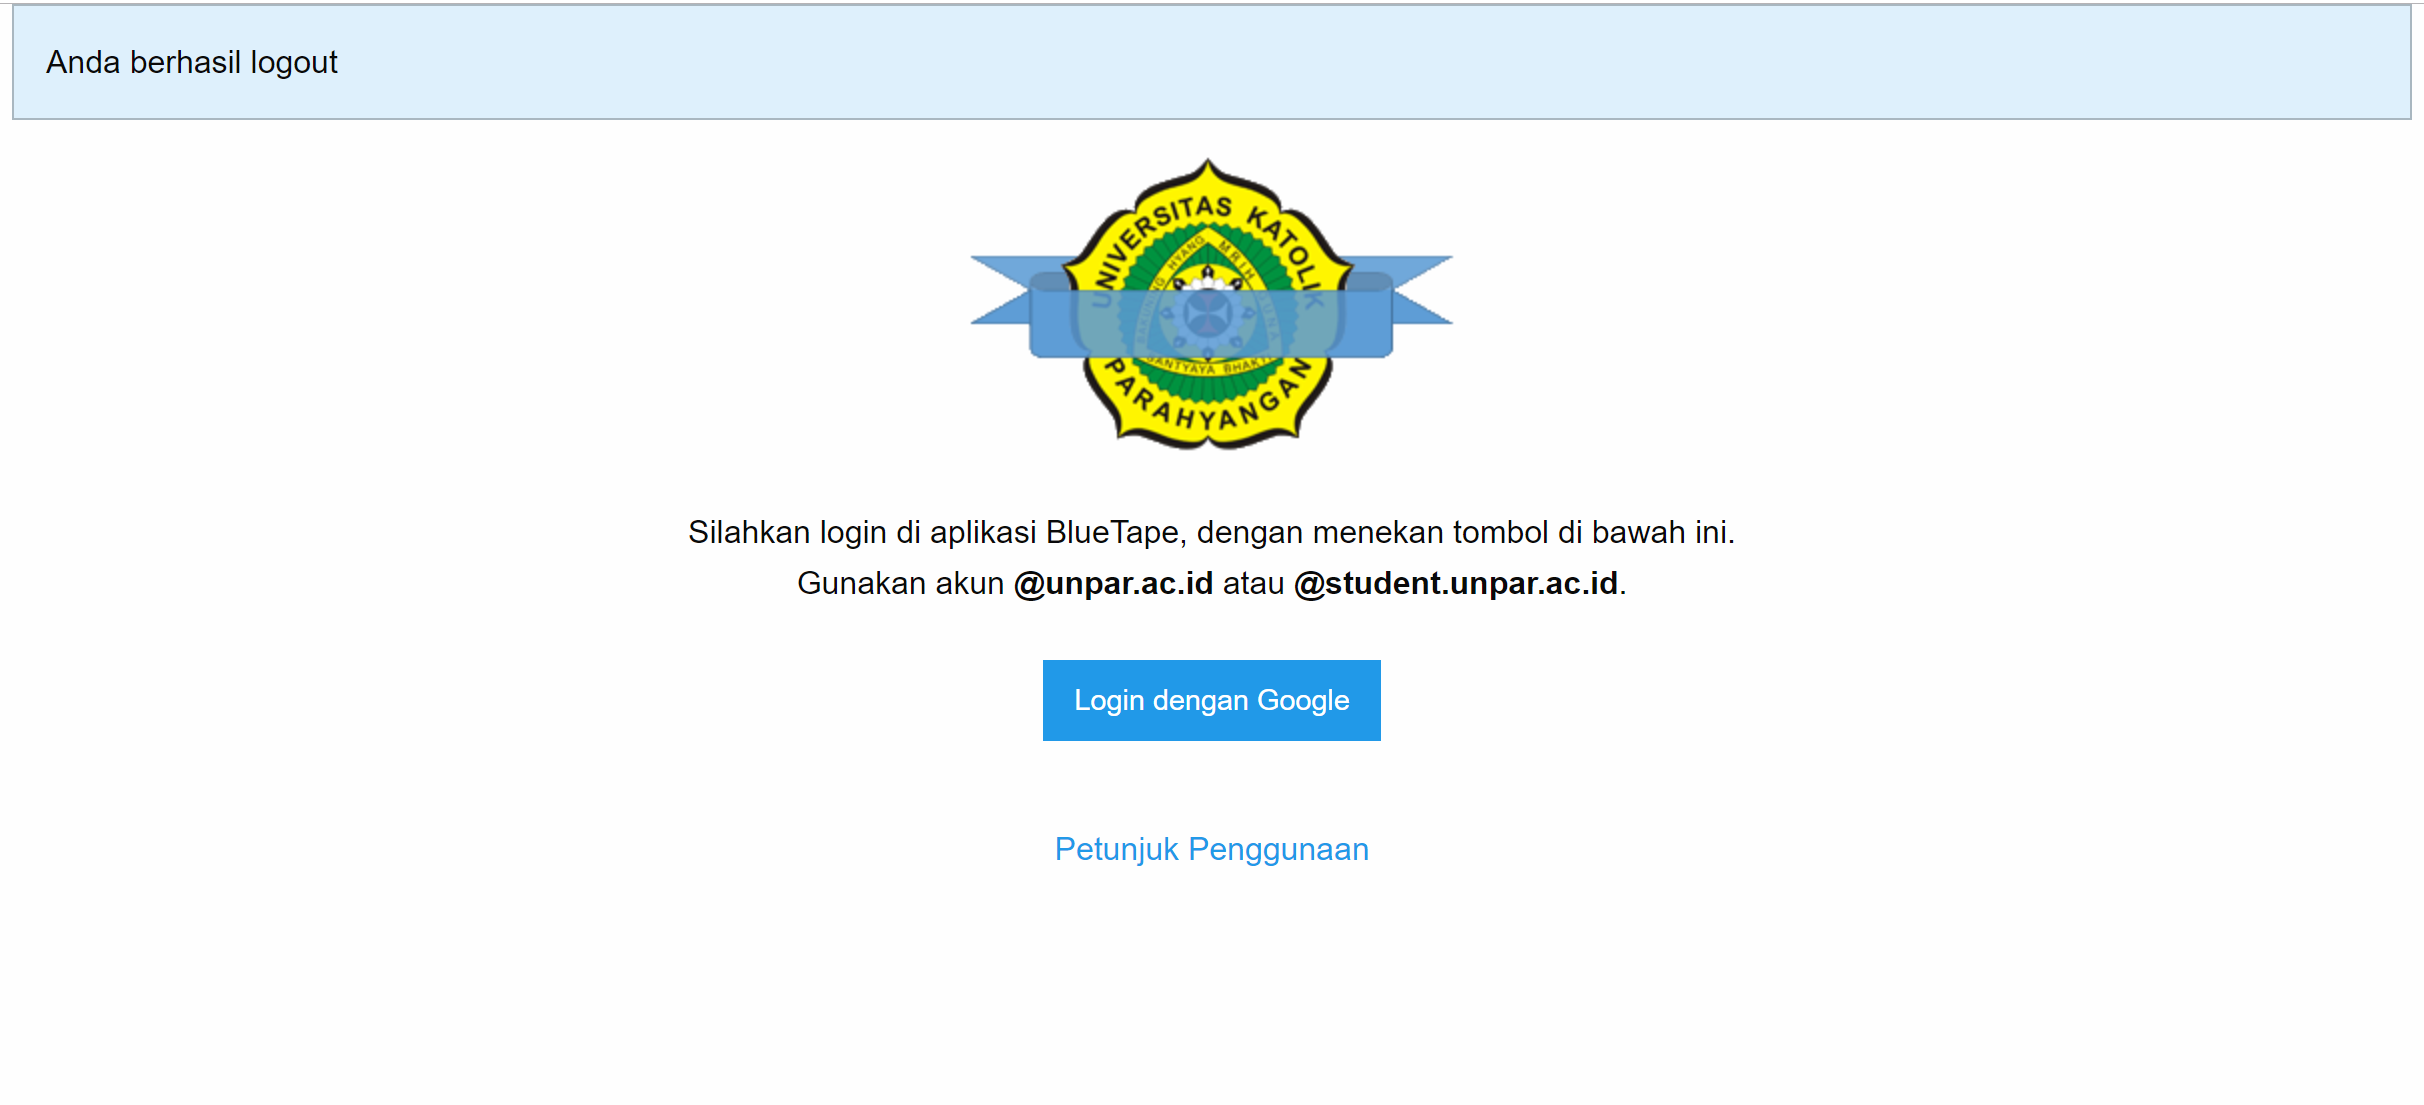
\includegraphics[scale=0.7]{alertInfo_zurb.png}  
	\caption{Alert mengenai 'info' pada BlueTape}	 
\end{figure}

\begin{figure} [H]
	\centering  
	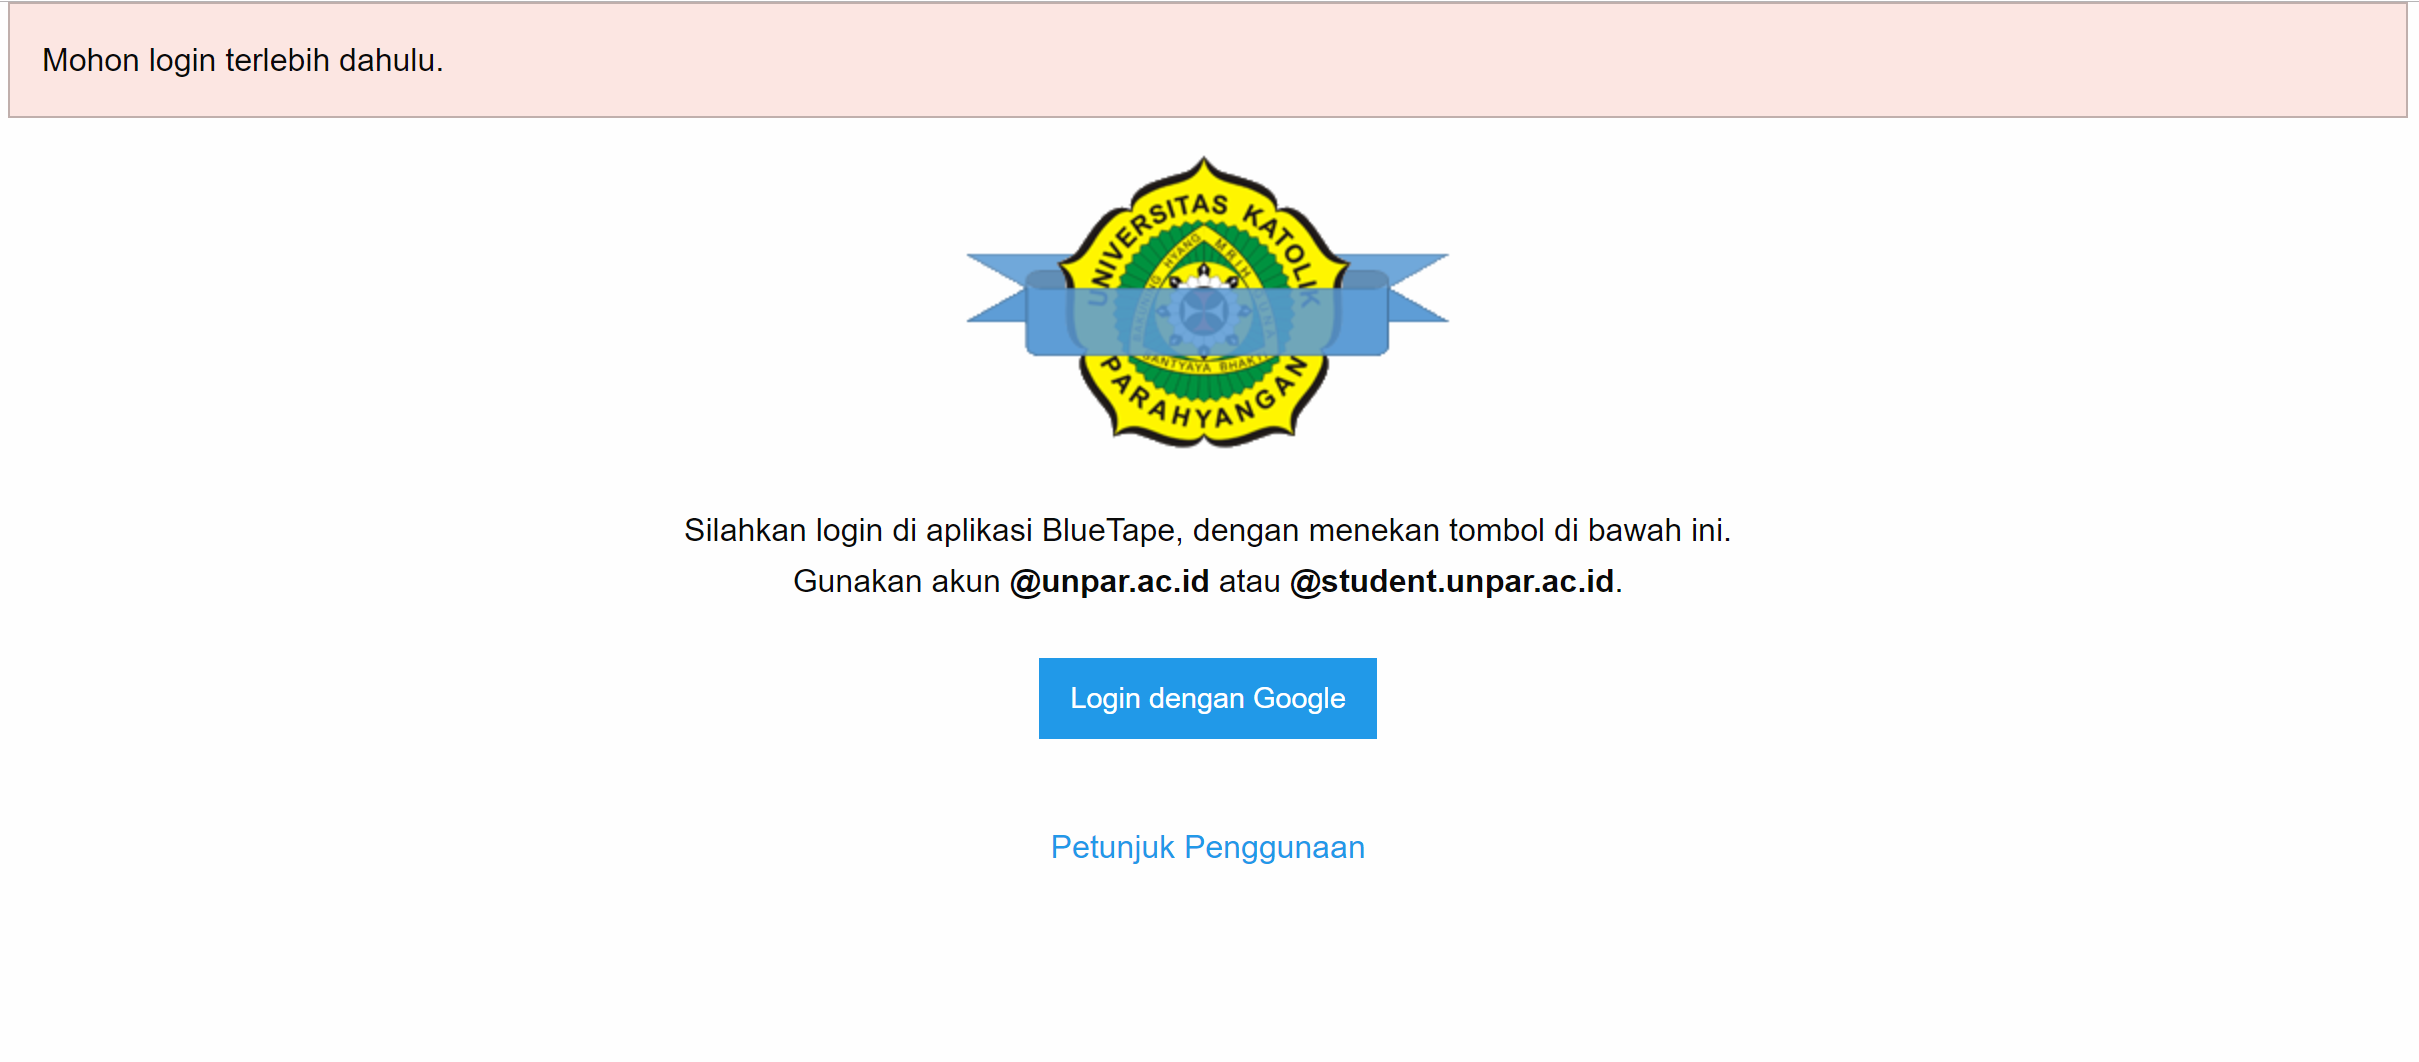
\includegraphics[scale=0.7]{alertError_zurb.png}  
	\caption{Alert mengenai 'error' pada BlueTape}	 
\end{figure}
\begin{enumerate}
	\item Alert 'error' : Penggunaan kelas \colorbox{mygray}{\texttt{callout error}} akan membuat komponen \textit{alert} berwarna merah.
	\item Alert 'info' : Penggunaan kelas \colorbox{mygray}{\texttt{callout alert}} akan membuat komponen \textit{alert} berwarna biru.
\end{enumerate}

\subsection{Template Head Logged In}
File ini terletak di \textbf{BlueTape/www/application/views/templates/head\_loggedin.php}.

\begin{figure} [H]
	\centering  
	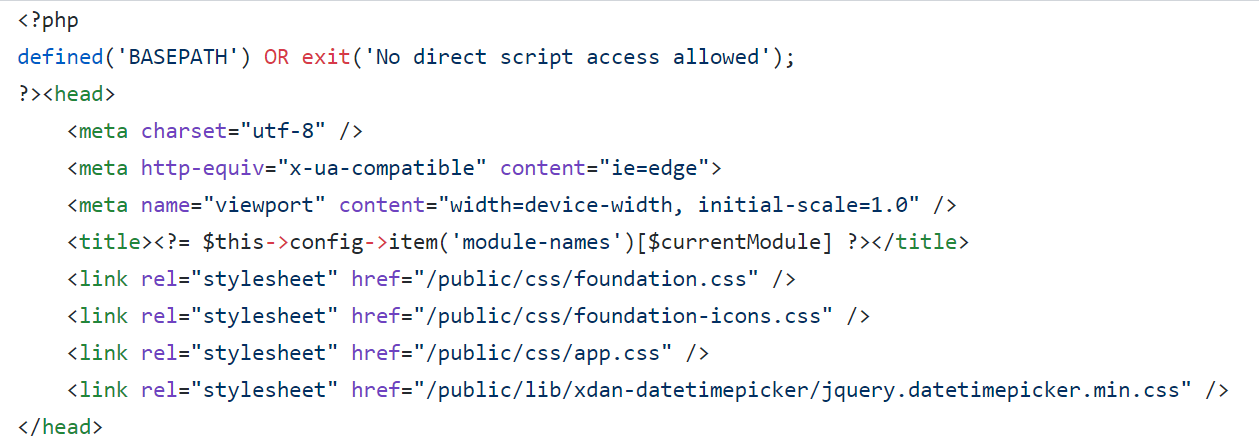
\includegraphics[scale=0.7]{head_loggedin.png}  
	\caption{Kode template untuk file head\_loggedin.php} 
\end{figure}

\subsection{Template Script Foundation}
File ini terletak di \textbf{BlueTape/www/application/views/templates/script\_loggedin.php}.
 
\begin{figure} [H]
	\centering  
	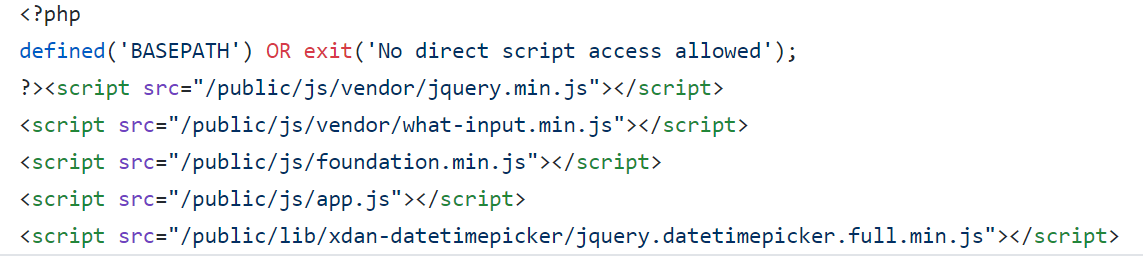
\includegraphics[scale=0.7]{script_foundation.png}  
	\caption{Kode template untuk file script_foundation.php} 
\end{figure}
\subsection{Template Top Bar Logged In}
File ini terletak di \textbf{BlueTape/www/application/views/templates/topbar\_loggedin.php}.
\begin{figure} [H]
	\centering  
	
\includegraphics[scale=0.7]{Tampilan_navbar_zurb.png}  
	\caption{Tampilan navbar dengan foundation} 
\end{figure}
\subsection{Antarmuka Cetak Transkrip}
Antarmuka diaplikasikan pada file \textbf{BlueTape/www/application/views/TranskripRequest/main.php}. Isi dari halaman antarmuka cetak transkrip terdiri dari dua bagian yaitu :
\begin{enumerate}
	\item \verb|Permohonan Baru| : Sistem akan memberikan dua tampilan untuk bagian ini, dengan kondisi sebagai berikut:
	\begin{itemize}
		\item Sistem akan menampilkan form pengajuan transkrip, apabila mahasiswa belum pernah mengajukan permohonan atau pengajuan sebelumnya  dikonfirmasi staf TU, maka mahasiswa dapat mengajukan permohonan baru.
		\item Sistem akan menampilkan informasi "Anda tidak bisa meminta cetak karena ada permintaan lain yang belum selesai", apabila mahasiswa memiliki pengajuan permohonan transkrip yang belum dikonfirmasi staf TU. 
	\end{itemize}
	\item \verb|Histori Permohonan| : Tabel untuk menampilkan informasi permohonan transkrip seorang mahasiswa. Status, tanggal pembuatan, tipe transkrip, tanggal cetak keterangan dan aksi. 
\end{enumerate}
Desain antarmuka sebagai berikut : \par
Konten 'Permohonan Baru' dan 'Histori Permohonan' akan diletakkan pada satu \textit{row} yang memiliki kolom sebesar 12 grid pada layar medium dengan menggunakan komponen \colorbox{mygray}{\texttt{medium-12 column}}, untuk setiap konten nya akan dipisahkan oleh panel yang disebut dengan \texttt{callout}. \par
Untuk konten Permohonan Baru :
\begin{itemize}
	\item Bagian isi akan memiliki dua tampilan yaitu berbentuk form atau notifikasi yang berbentuk paragraf. Sehingga dibutuhkan komponen \verb|<form>| dan \verb|<p>|.
	\item Form terdiri dari dua baris yang dipisahkan oleh komponen \texttt{row}.
	\item Untuk field pada baris pertama akan memiliki kolom dengan panjang 4 grid. Sehingga dibutuhkan kelas \verb|large-4 column|. Jenis input yang digunakan bertipe email dan text. Selain itu untuk setiap input akan disertakan satu label sehingga menggunakan komponen \texttt{<label>}.
	\item Untuk field pada baris kedua memiliki dua jenis lebar grid yaitu 4 grid dan 8 grid. Sehingga membutuhkan kelas \verb|large-4 column|, \verb|large-8 column|. Untuk fied pada baris ketiga, tombol "Kirim Permohonan" memiliki \textit{background color} berwarna biru sehingga akan digunakan kelas \verb|button|.
\end{itemize}
Untuk konten "Histori Permohonan" :
\begin{enumerate}	
	\item Pada kolom "Status" akan memiliki tiga jenis bentuk alert dengan \textit{backgroud} warna hijau, abu-abu dan merah. Sehingga dibutuhkan kelas \verb|warning|, \verb|success|, \verb|alert|.
	\item Aksi memiliki satu ikon "lihat" berwarna biru yang akan menampilkan sebuah modal. Sehingga dibutuhkan kelas ikon \verb|fi-eye|.
\end{enumerate}
\begin{figure} [H]
	\centering  
	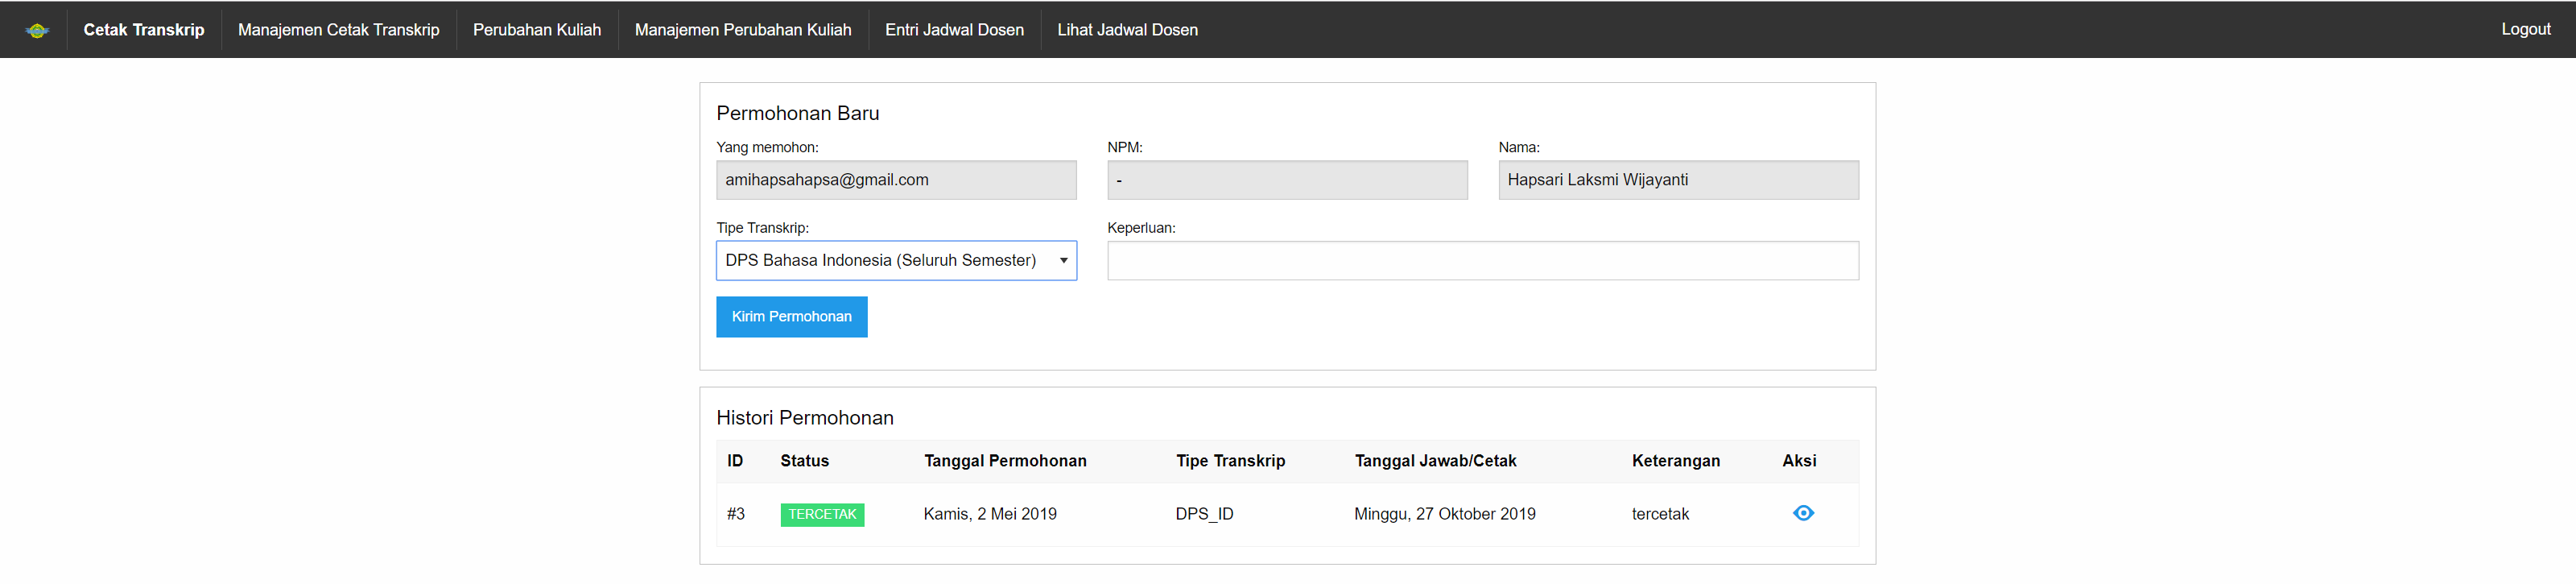
\includegraphics[scale=0.5]{Tampilan-Mahasiswa-Cetak-Transkrip.png}  
	\caption{Antarmuka Cetak Transkrip bagian 1} 
\end{figure}
\begin{figure} [H]
	\centering  
	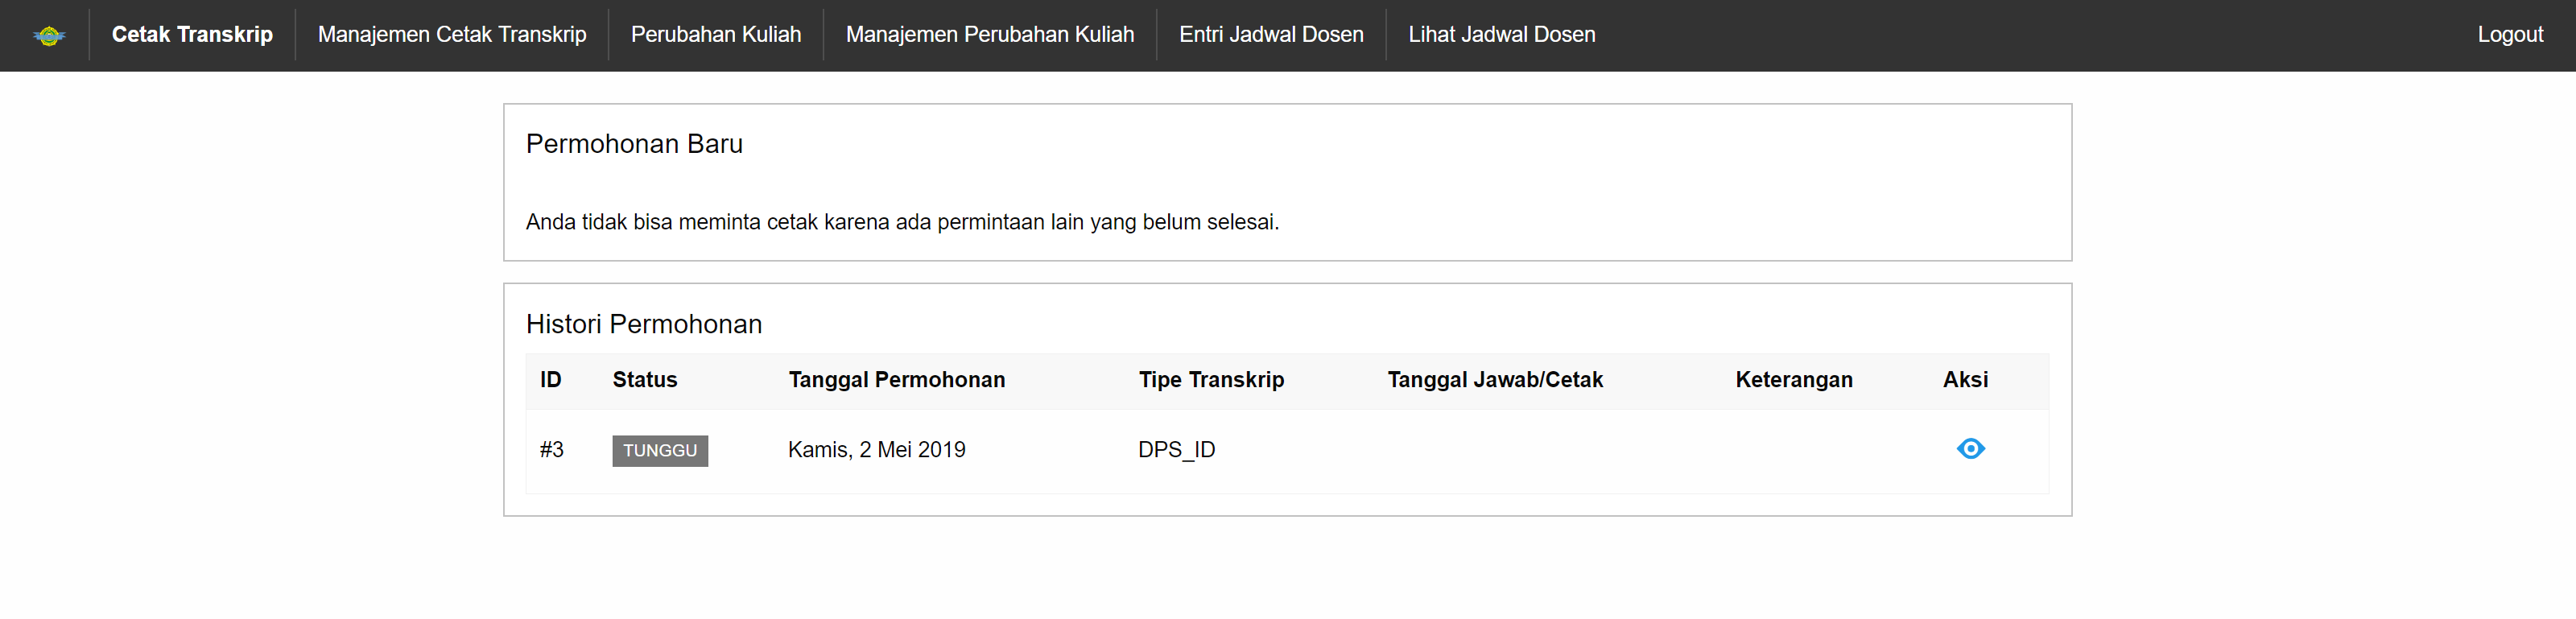
\includegraphics[scale=0.5]{Tampilan-Cetak-Transkrip.png}  
	\caption{Antarmuka Cetak Transkrip bagian 2} 
\end{figure}
Detail dari form permohonan baru, semua field akan disertai sebuah label untuk menjelaskan fungsi setiap field sehingga membutuhkan tag \texttt{<label>}  :
\begin{itemize}	
	\item \texttt{Yang memohon} : Berisi email UNPAR mahasiswa, otomatis terisi saat login melalui gmail. Sehingga field tidak bisa diisi atau \textit{disabled} dibutuhkan atribut boolean \verb|readonly|
	\item \texttt{NPM} : Berisi NPM mahasiswa yang ter-\textit{generate} secara otomatis. Sehingga field tidak bisa diisi atau \textit{disabled} dibutuhkan atribut boolean \verb|readonly| dan \texttt{<input>} dengan tipe text.
	\item \texttt{Nama} : Nama mahasiswa yang tergenerate secara otomatis. Sehingga field tidak bisa diisi atau \textit{disabled} dibutuhkan atribut boolean \verb|readonly| dan \texttt{<input>} dengan tipe text.
	\item \texttt{Tipe Transkrip} : Terdiri dari tiga pilihan yaitu DPS Bahasa Indonesia(Seluruh Semester), DPS Bahasa Inggris(Seluruh Semester), LHS (Semester Terakhir). Wajib diisi. Tag \texttt{<select>} dan \texttt{<option>} yang \textit{value} nya diambil dari varibel \$type.
	\item Keperluan : Keterangan keperluan dibuat nya transkrip, wajib diisi mahasiswa. Menggunakan tag \texttt{<input>} dengan tipe text.
\end{itemize}
Apabila ada form yang belum diisi maka akan terdapat \textit{warning} untuk \textit{field} yang kosong.
Berikut ini apabila mahasiswa menekan tombol aksi lihat 
\includegraphics[height=0.7\baselineskip]{tombol_eye.png} :
\begin{figure} [H]
	\centering  
	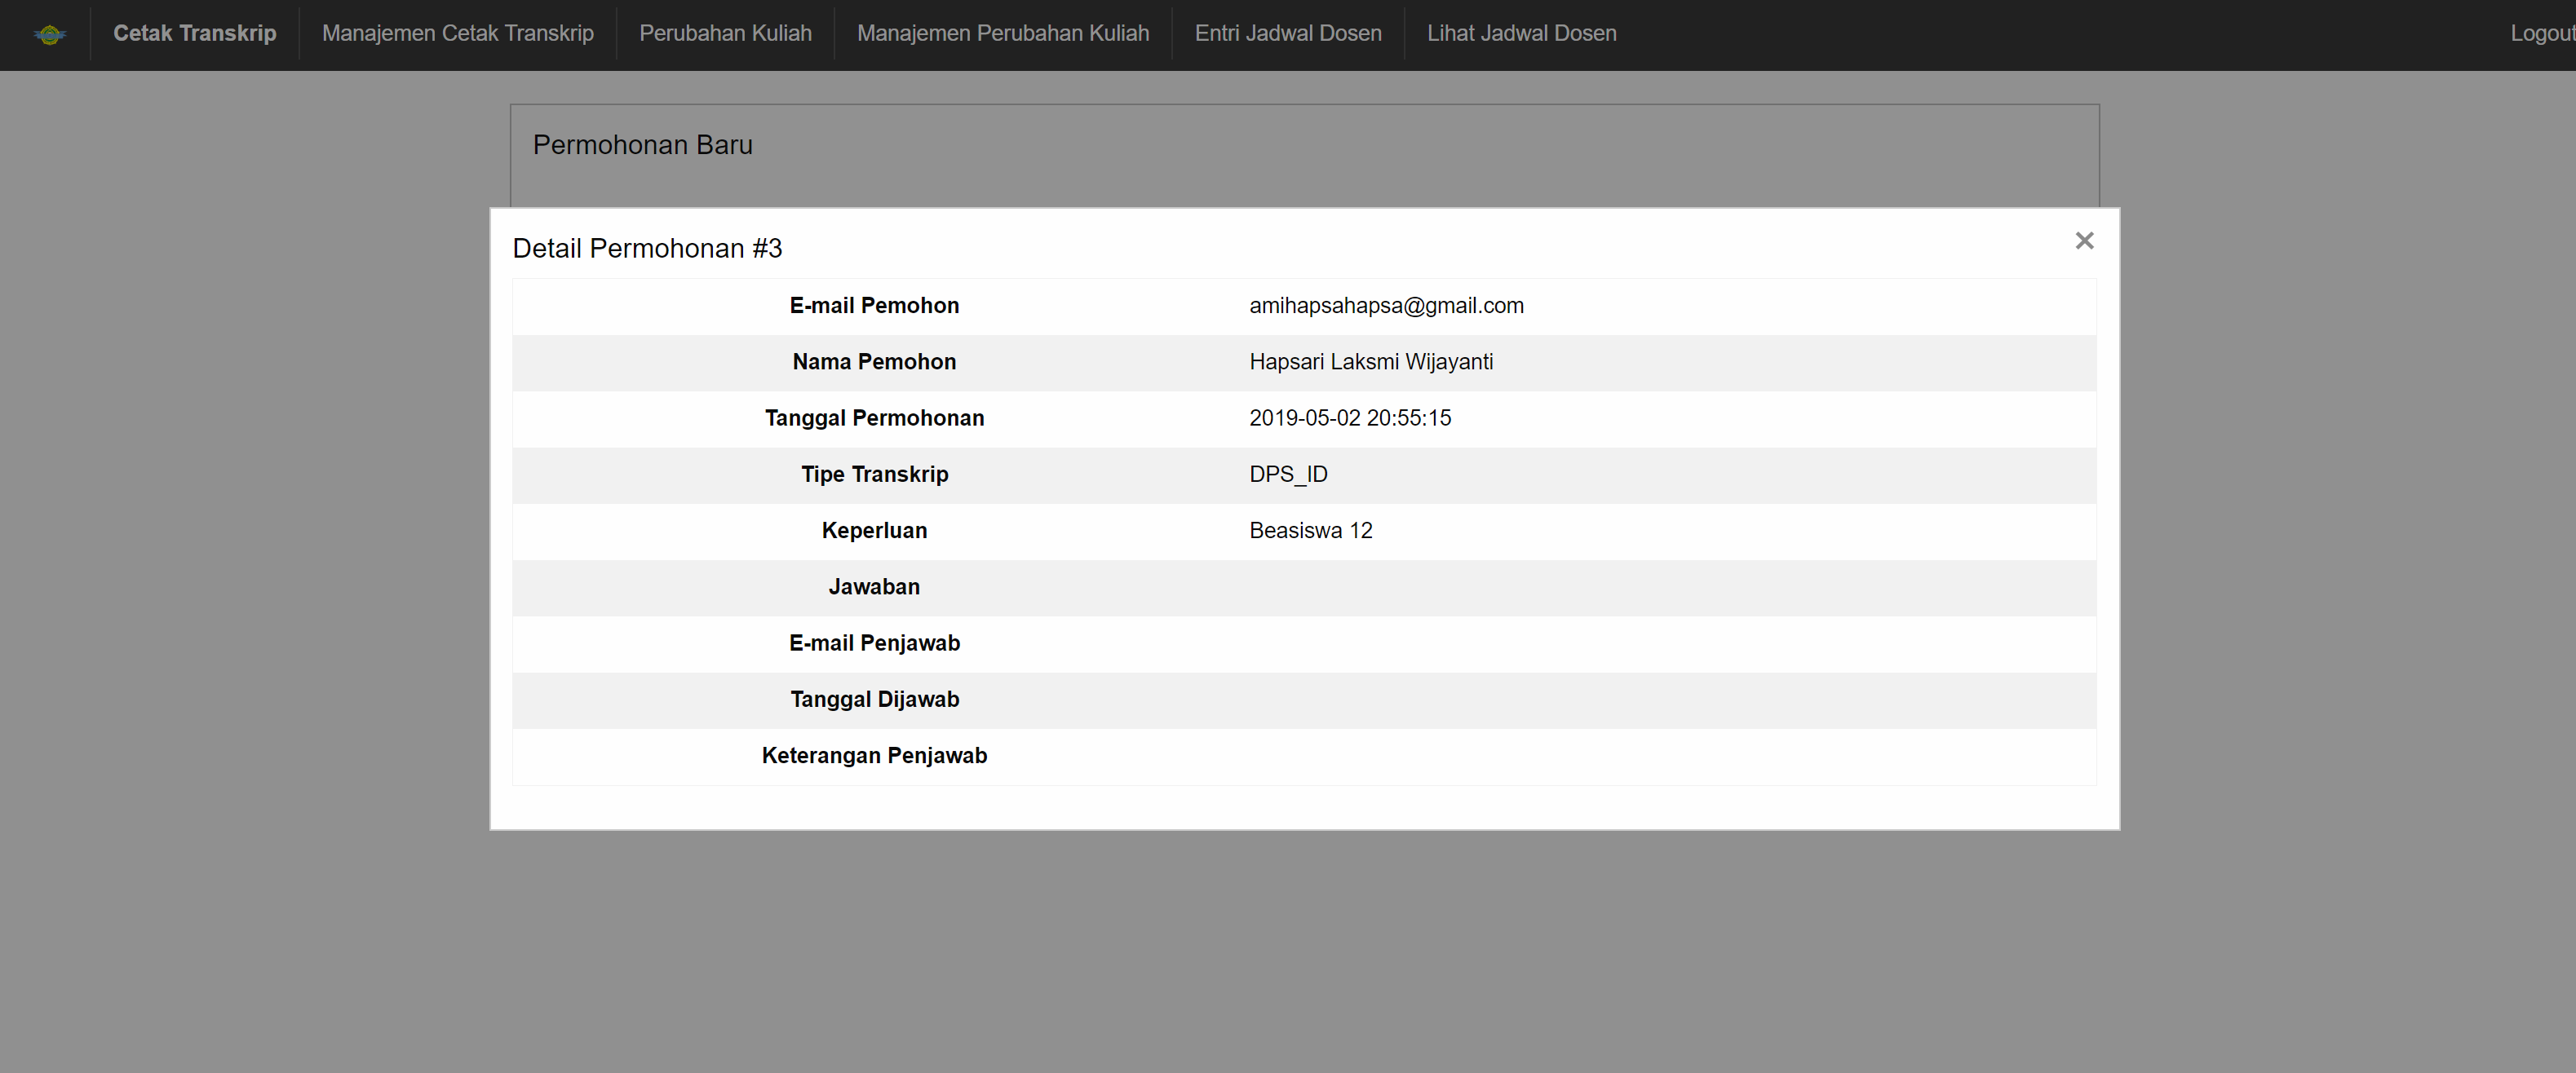
\includegraphics[scale=0.5]{Modal-Lihat-Cetak-Transkrip.png}  
	\caption{Modal Lihat Cetak Transkrip} 
\end{figure}
\noindent Disini aksi 'lihat' akan menampilkan sebuah modal yang berisi sebuah tabel bergaris yang menyimpan informasi detil permohonan, baik detil informasi dari mahasiswa maupun konfirmasi dari staf Tata Usaha. Sehingga dibutuhkan kelas \verb|.reveal| dan atribut \verb|data-reveal|.

\subsection{Antarmuka Manajemen Cetak Transkrip}
Antarmuka diaplikasikan pada file \textbf{BlueTape/www/application/views/TranskripManage/main.php}.
\begin{figure} [H]
	\centering  
	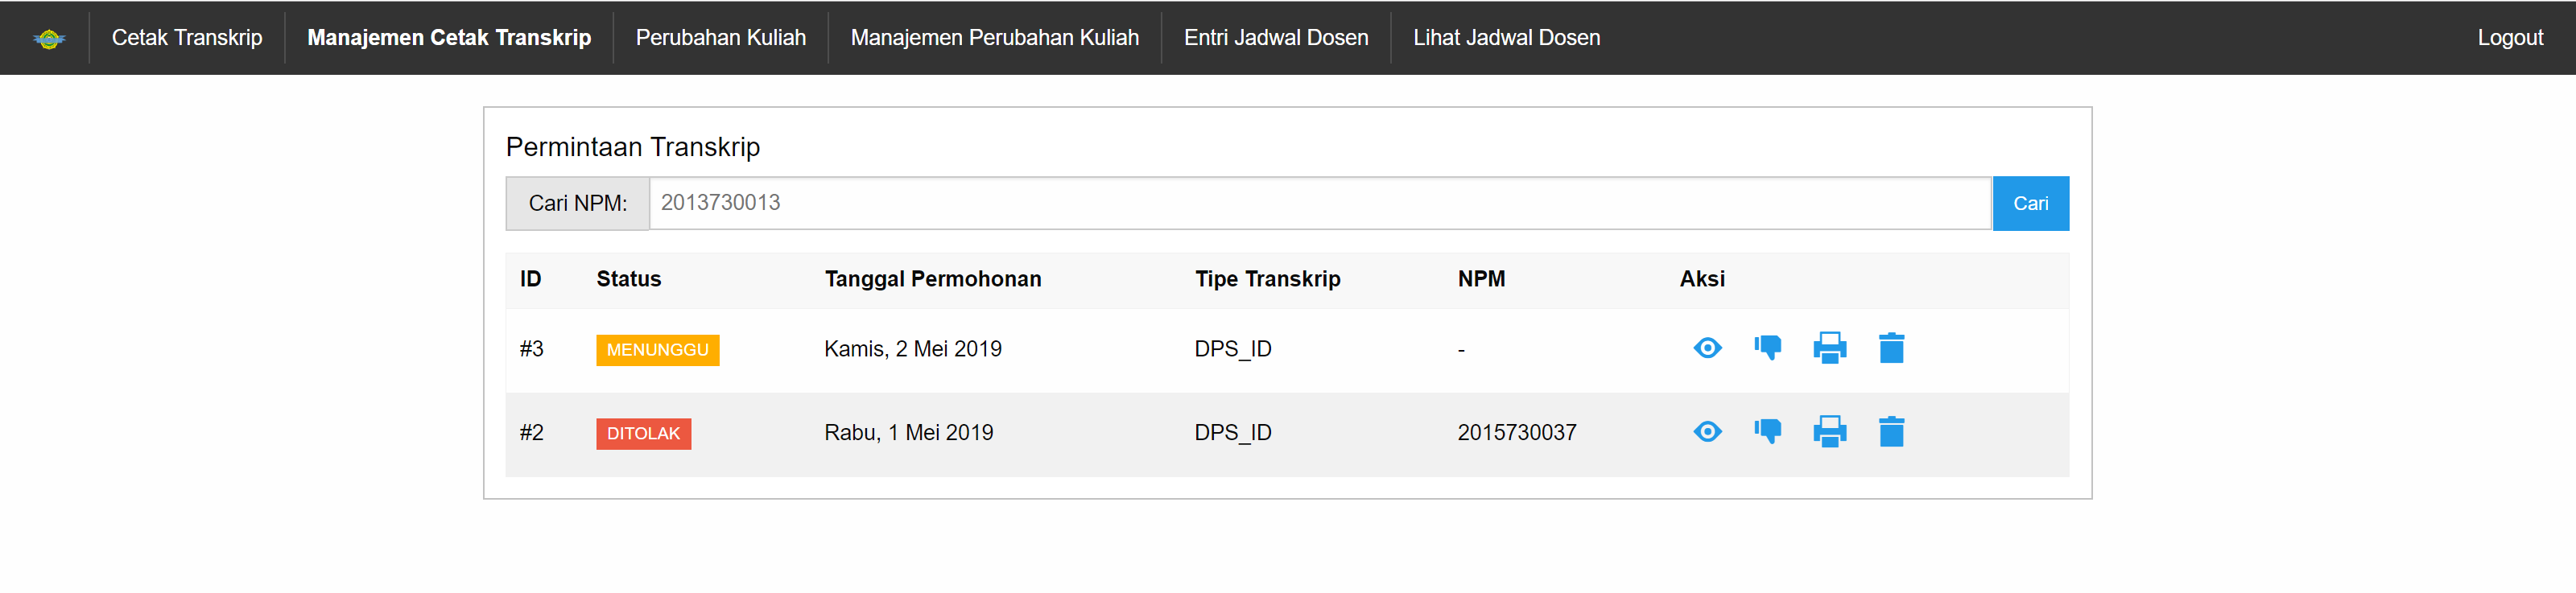
\includegraphics[scale=0.5]{Tampilan-Manajemen-Cetak-Transkrip.png}  
	\caption{Tampilan Manajemen Cetak Transkrip} 	
\end{figure}

Tampilan Manajemen Cetak Transkrip berisi sebuah tabel permintaan transkrip yang terdiri dari daftar permintaan transkrip dan form pencarian transkrip berdasarkan NPM. \par

\noindent Detail penjelasan untuk field 'Status' dan 'Aksi' :
\begin{itemize}
	\item \texttt{Status} : Output terdiri dari tiga jenis label yaitu 'MENUNGGU'(berwarna kuning), 'DITOLAK' (berwarna merah) dan 'TERCETAK'(berwarna hijau).  Sehingga dibutuhkan kelas \colorbox{mygray}{\verb|secondary|}, \colorbox{mygray}{\verb|success|}, \colorbox{mygray}{\verb|alert|}. 
	\item \texttt{Aksi} : Terdiri dari empat ikon font-awesome yaitu \verb|fi-eye, fi-dislike, fi-print, fi-trash,| yang akan menampilkan modal berisi informasi yang sesuai dengan perintah.
\end{itemize}
Modal akan menggunakan kelas \texttt{reveal} dan atribut \texttt{data-reveal} Detail penjelasan untuk modal : 

\begin{enumerate}
	
	\item Modal Lihat : Terdiri dari sebuah \texttt{table} yang menampilkan data permintaan transkrip. Ikon menggunakan kelas \texttt{fi-eye} dan menerapkan atribut \texttt{data-open} yang berisi method hapus menuju ID tertentu.
	
	\item Modal Tolak : Terdiri dari sebuah \texttt{form} yang memiliki method \texttt{POST} yang memanggil sebuah method "/TranskripManage/answer". Terdapat tiga tipe input yang digunakan yaitu \texttt{hidden, text, submit}. Pada input text untuk label Alasan Penolakan, menggunakan kelas "input-group-field". Lalu untuk input bertipe \texttt{submit} menggunakan kelas alert-button untuk membuat button berwarna merah. Ikon menggunakan kelas \texttt{fi-dislike} dan menerapkan atribut \texttt{data-open} yang berisi method tolak menuju ID tertentu.
	
	\item Modal Print : Terdiri dari sebuah form yang terdiri dari label, field dan tombol berwarna biru sehingga membutuhkan kelas \colorbox{mygray}{\verb|input-group-field|}. Ikon menggunakan kelas \colorbox{mygray}{\texttt{fi-print}} dan menerapkan atribut \colorbox{mygray}{\texttt{data-open}} yang berisi method cetak menuju ID tertentu.
	
	\item Modal Hapus : Terdiri dari sebuah form yang terdiri dari paragraf yang bersifat bold, beberapa input dan tombol berwarna merah sehingga membutuhkan kelas \colorbox{mygray}{\verb|<p>|}, \colorbox{mygray}{<strong>}},\colorbox{mygray}{\texttt{<input>}}.Ikon menggunakan kelas \texttt{fi-trash} dan menerapkan atribut \texttt{data-open} yang berisi method hapus menuju ID tertentu.
\end{enumerate}

\begin{figure} [H]
	\centering  
	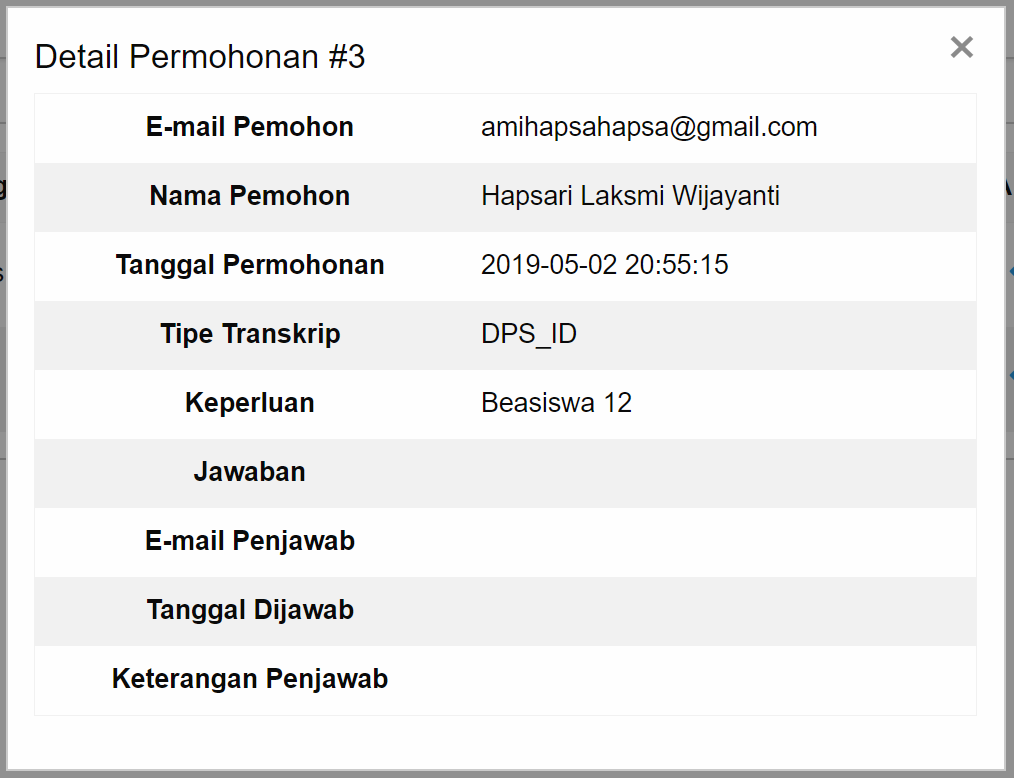
\includegraphics[scale=0.5]{Modal-Lihat-Manajemen-Cetak-Transkrip.png}  
	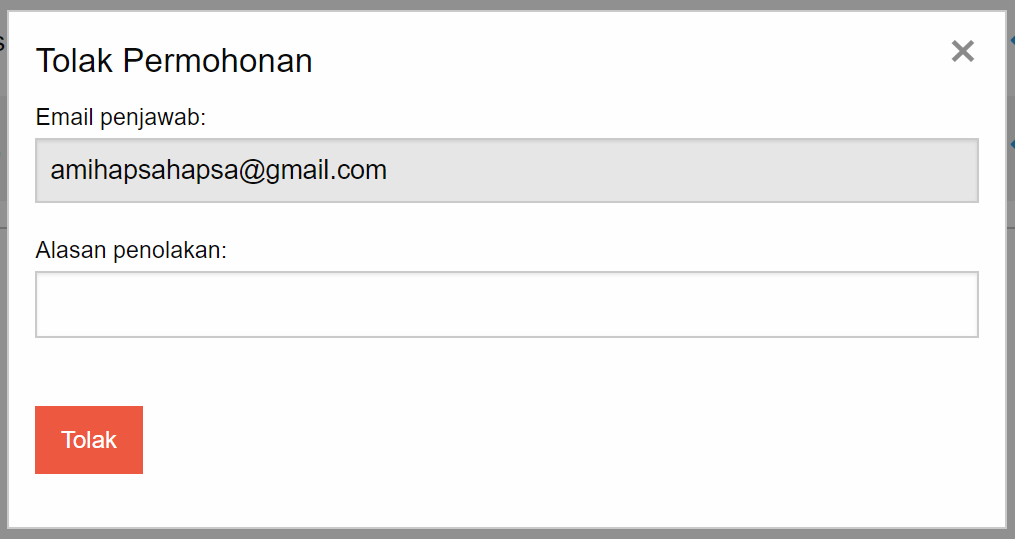
\includegraphics[scale=0.5]{Modal-Tolak-Manajemen-Cetak-Transkrip.png} 
	\caption{Tampilan Modal untuk aksi 'Lihat' dan 'Tolak'} 	
\end{figure}

\begin{figure} [H]
	\centering  
	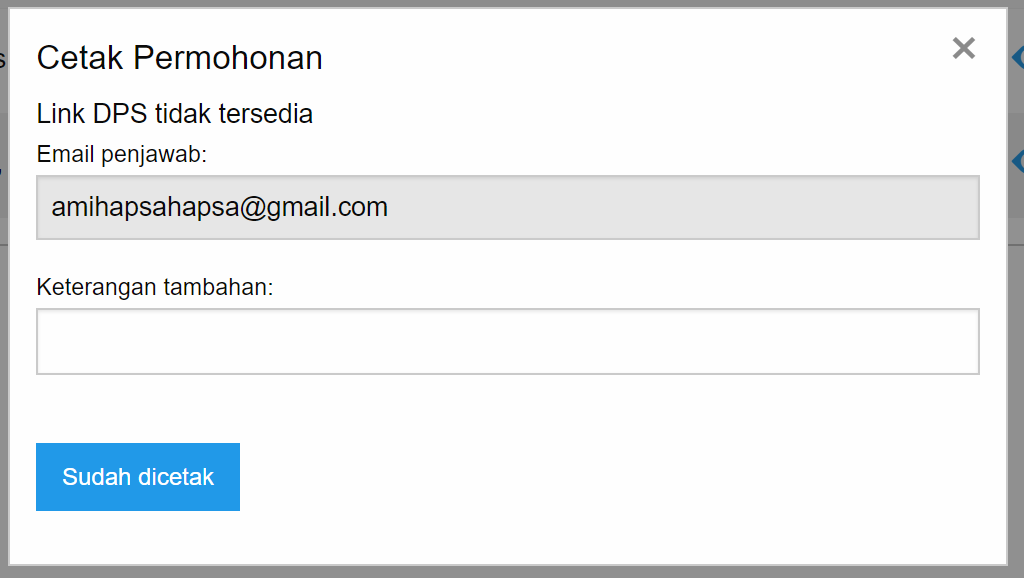
\includegraphics[scale=0.5]{Modal-Print-Manajemen-Cetak-Transkrip.png}  
	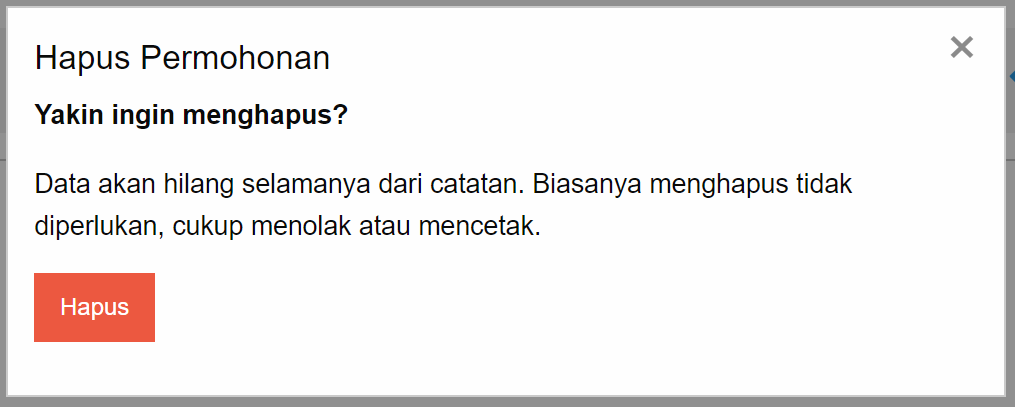
\includegraphics[scale=0.5]{Modal-Hapus-Manajemen-Cetak-Transkrip.png} 
	\caption{Tampilan Modal untuk aksi 'Print' dan 'Hapus'} 	
\end{figure}


\subsection{Antarmuka Perubahan Kuliah}
Antarmuka diaplikasikan pada file \textbf{BlueTape/www/application/views/PerubahanKuliahRequest/main.php}.
\begin{figure} [H]
	\centering  
	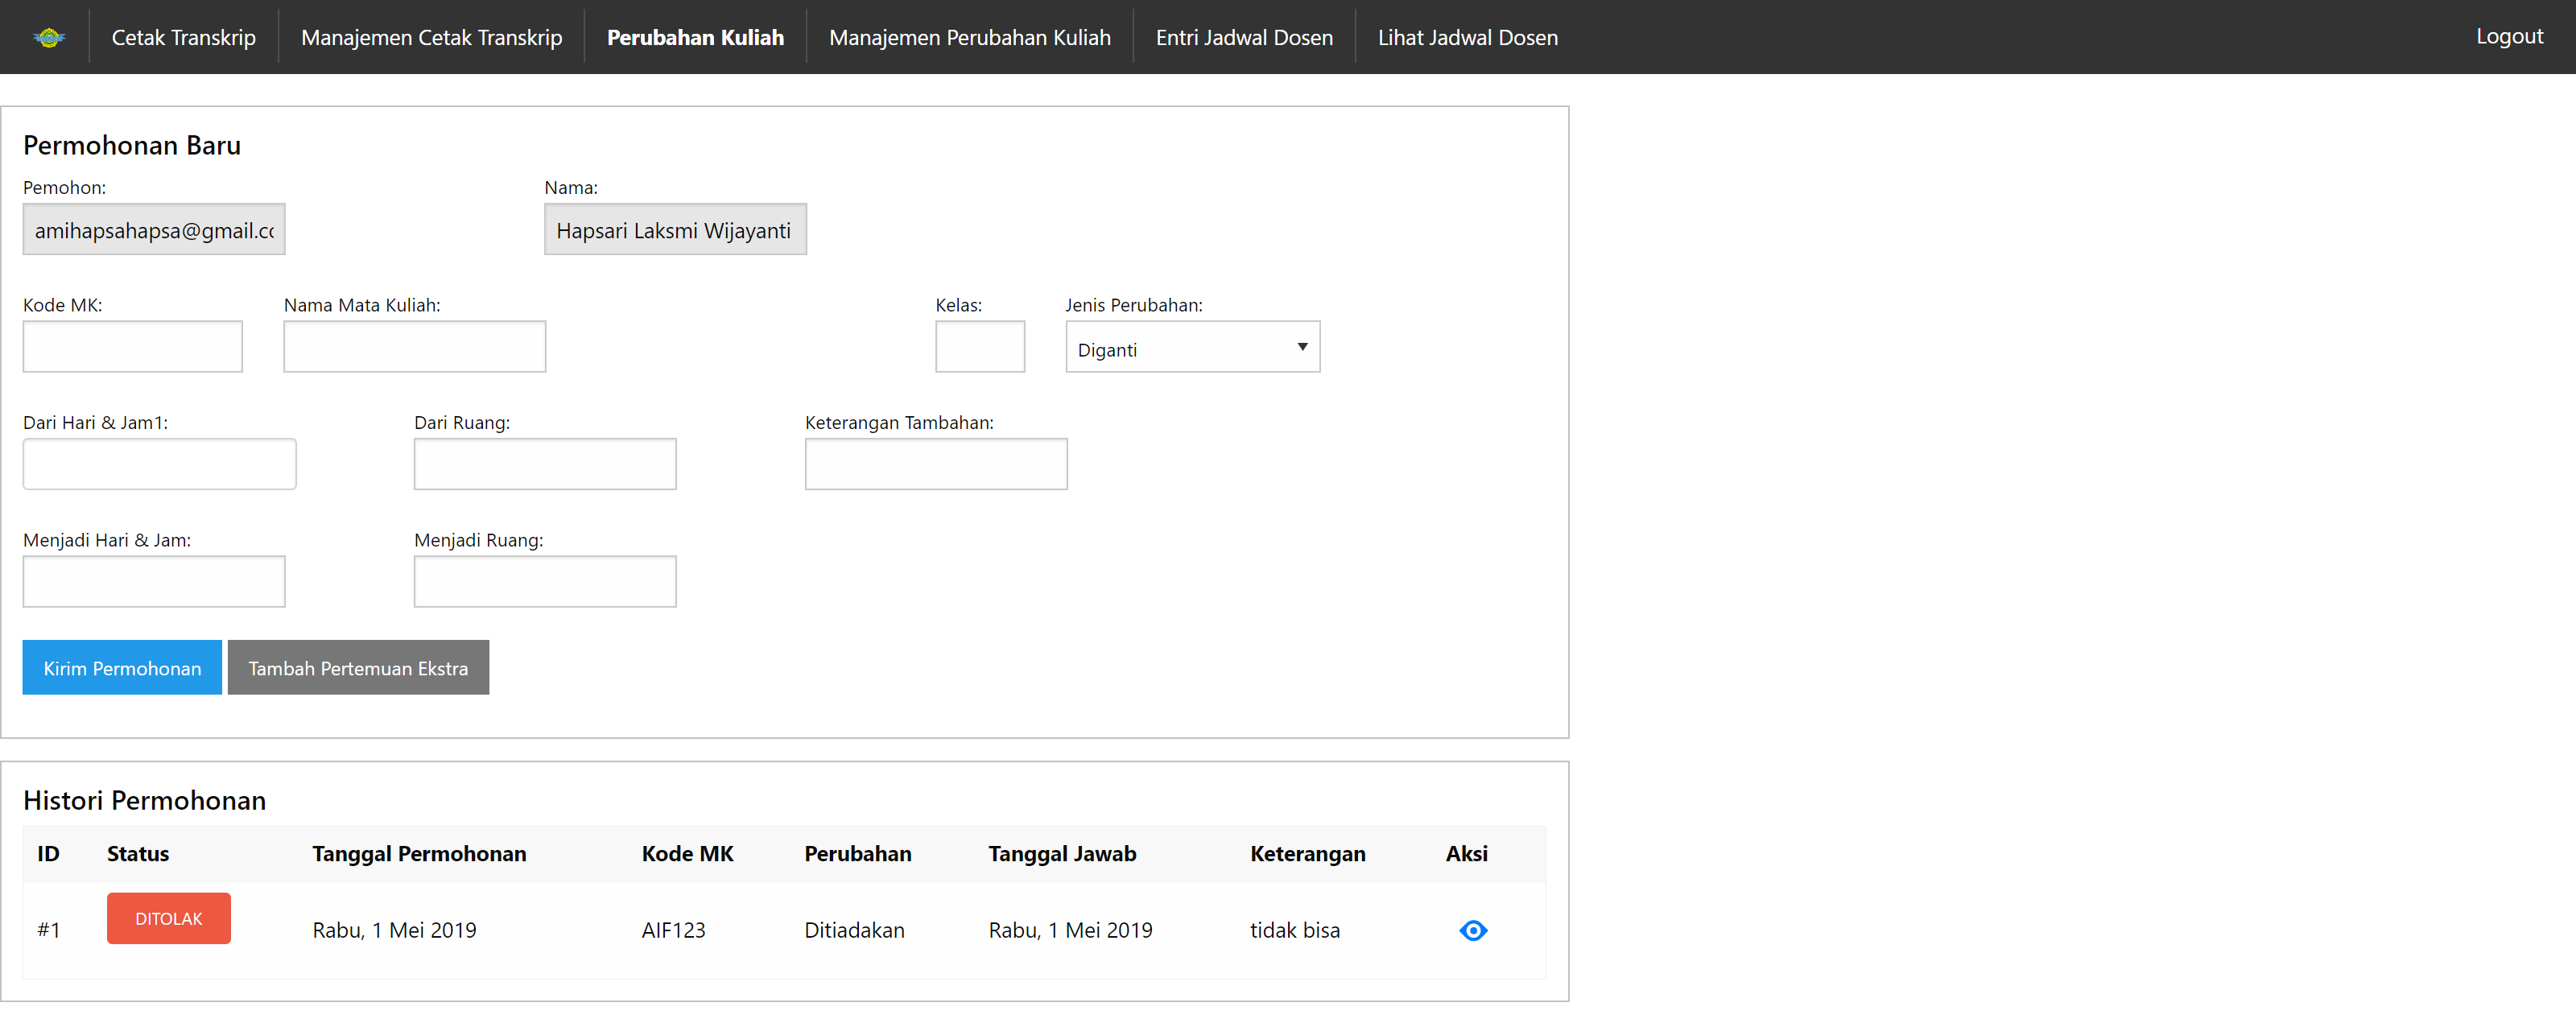
\includegraphics[scale=0.5]{Tampilan-Perubahan-Kuliah.png}  
	\caption{Tampilan Perubahan Kuliah} 
\end{figure}
Modul Perubahan Kuliah terdiri dari dua tabel yaitu :


\subsection{Permohonan Baru}
Permohonan baru diletakkan dalam sebuah row selebar 12 grid dan dikelilingi oleh sebuah border, membutuhkan kelas \colorbox{mygray}{\texttt{row, large-12 column}} dan \texttt{callout}. Selain itu sebuah form dengan tipe \texttt{POST} akan ditampilkan untuk menyimpan masukan pemohon. Format dari form sebagai berikut :



\subsection{Histori Pemohonan}
Histori Permohonan menggunakan tabel yang bisa menyesuaikan lebarnya dengan menampilkan data secara bertumpuk sehingga menggunakan kelas \colorbox{mygray}{\texttt{.stack}}. Jenis data akan diletakkan dalam tag \\colorbox{mygray}{texttt{<thead>}} dalam satu baris sehingga menggunakan satu tag \colorbox{mygray}{\texttt{<tr>}} dan\texttt{delapan} tag \colorbox{mygray}{\texttt{<th>}}. Untuk bagian isi data menggunakan tag \colorbox{mygray}{\texttt{<tbody>}}.

\begin{tabular}[!htbp]{ |p{4cm}|p{2cm}|p{10cm}|  }
	\hline
	Nama Kolom & Pilihan & Kelas Foundation yang digunakan\\
	\hline
	\texttt{Status} & dikonfirmasi, menggunakan kelas \colorbox{mygray}{\verb|success|} & Apabila staf TU menyetujui permohonanan\\
	\hline
	&  ditolak, menggunakan kelas \colorbox{mygray}{\verb|alert|}  & Apabila staf TU menolak permohonanan\\
	\hline
	& ditunggu, menggunakan kelas \colorbox{mygray}{\verb|secondary|} &  Apabila staf TU belum konfirmasi permohonan \\
	\hline
	\texttt{Tanggal Permohonan}    & & Data bertipe tanggal dengan format yang sudah ditentukan\\
	\hline
	\texttt{Kode MK} &  & Data berbentuk text \\
	\hline
	\texttt{Perubahan} &  & Data berbentuk text \\
	\hline
	\texttt{Tanggal Jawab} &  & Data bertipe tanggal \\
	\hline
	\texttt{Keterangan} &  & Data berbentuk text \\
	\hline
	\texttt{Aksi} &  & Terdapat tombol aksi 'Lihat', menggunakan font awesome dan kelas \colorbox{mygray}{\verb|fas fa-eye|} yang akan memanggil sebuah modal sesuai id yang diinginkan user. Untuk modal, menggunakan kelas \texttt{reveal} dan atribut \colorbox{mygray}{\texttt{data-reveal}}\\
	\hline
\end{tabular}
Ketika user menekan tombol aksi 'lihat', maka modal berisi sebuah tabel informasi data permohonan akan ditampilkan sesuai dengan ID.
\begin{figure} [H]
	\centering  
	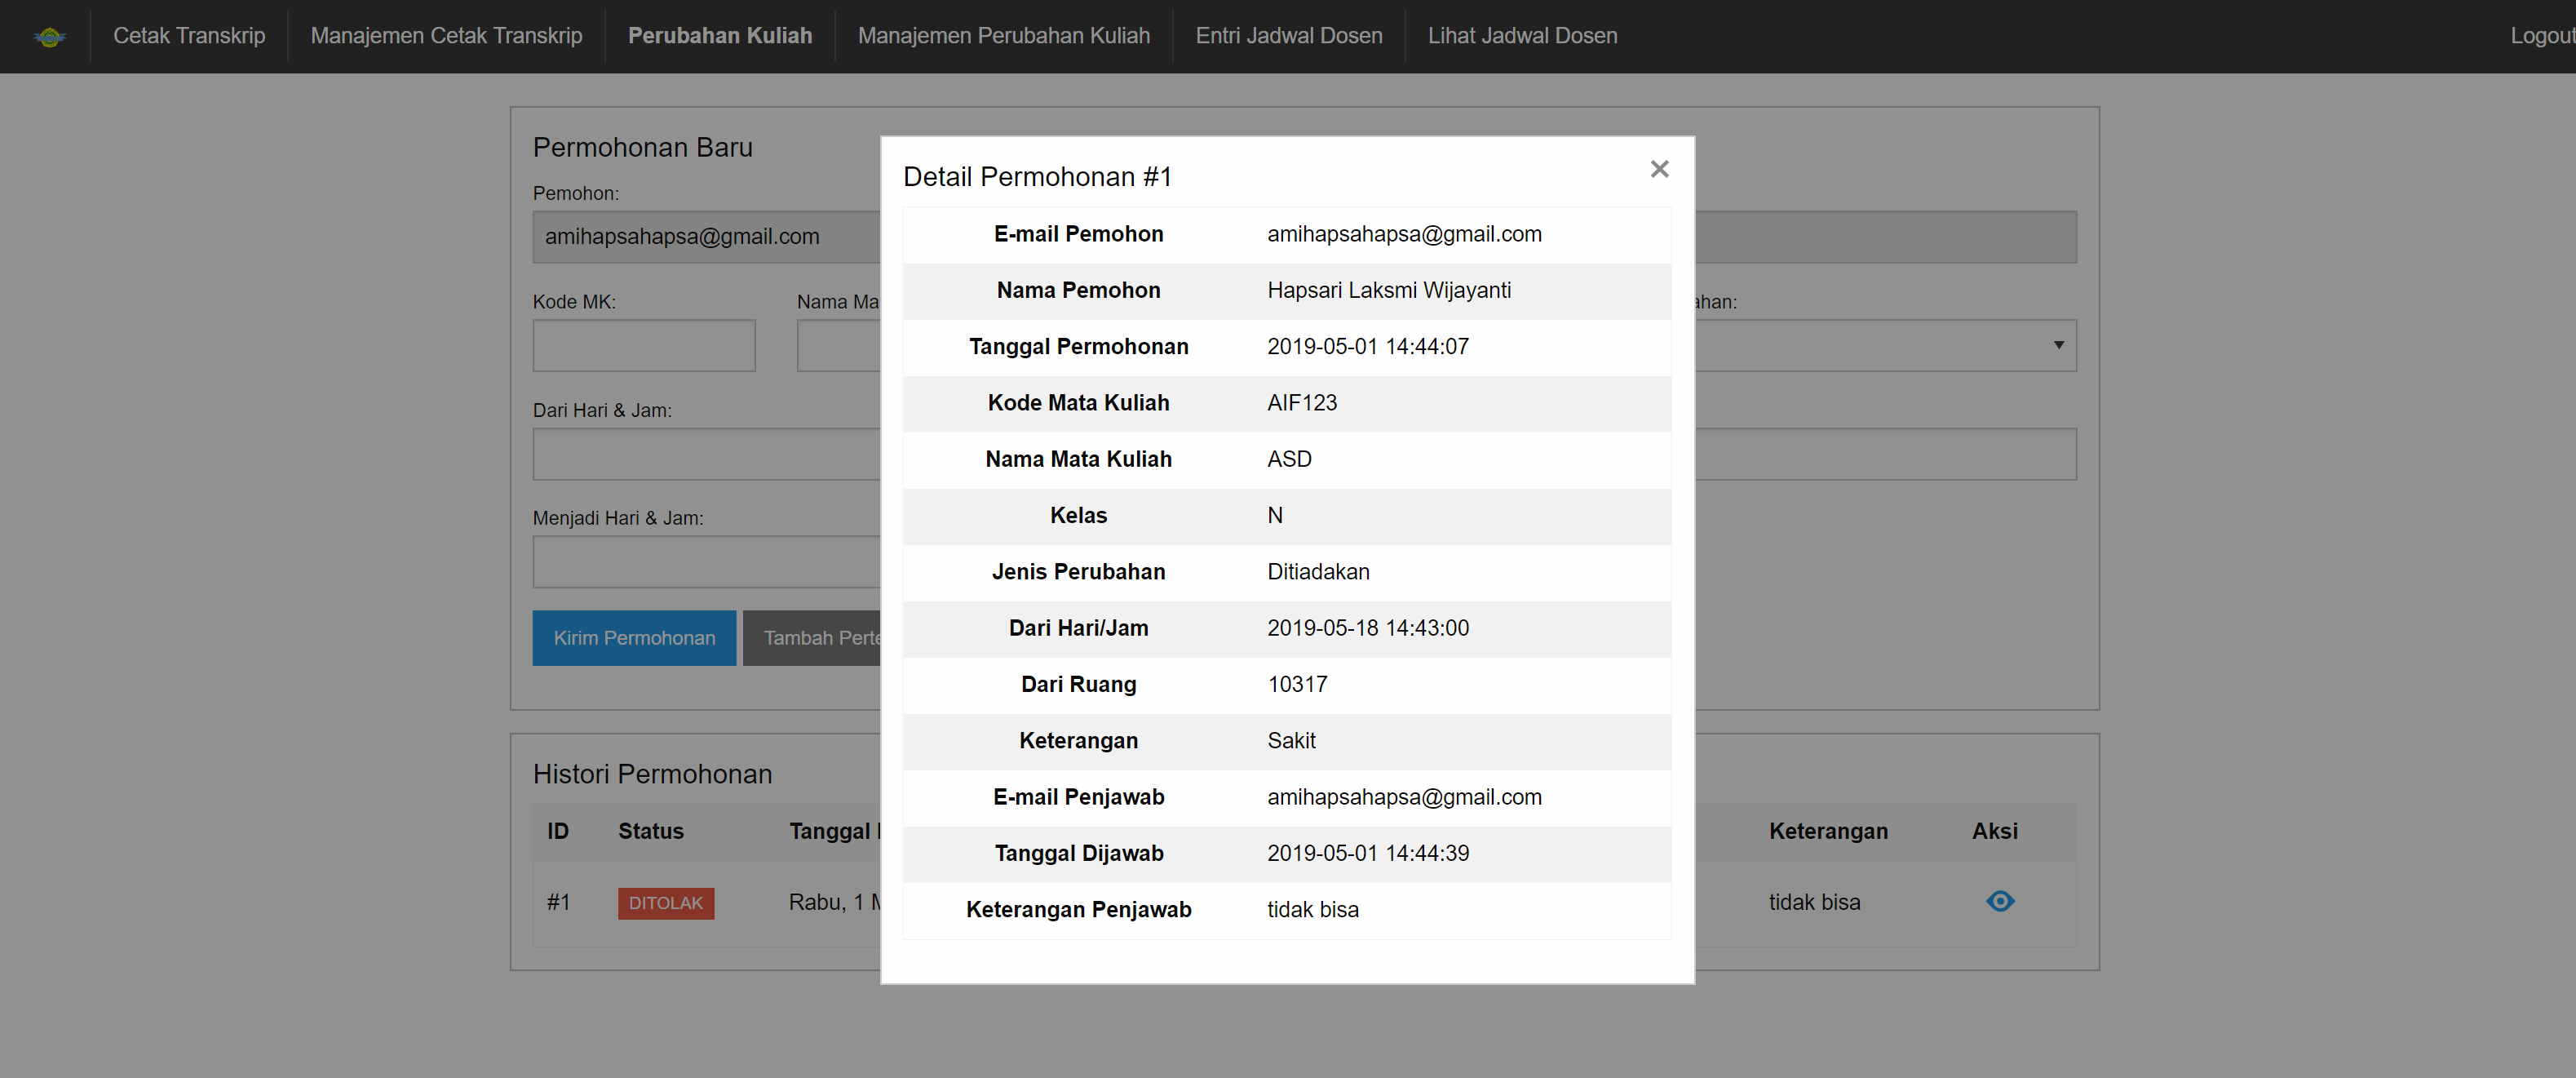
\includegraphics[scale=0.5]{Modal-Lihat-Perubahan-Kuliah.png}  
	\caption{Modal Lihat Perubahan Kuliah} 
\end{figure}

\subsection{Antarmuka Manajemen Perubahan Kuliah}
Antarmuka diaplikasikan pada file \textbf{BlueTape/www/application/views/PerubahanKuliahManage/main.php}.
\begin{figure} [H]
	\centering  
	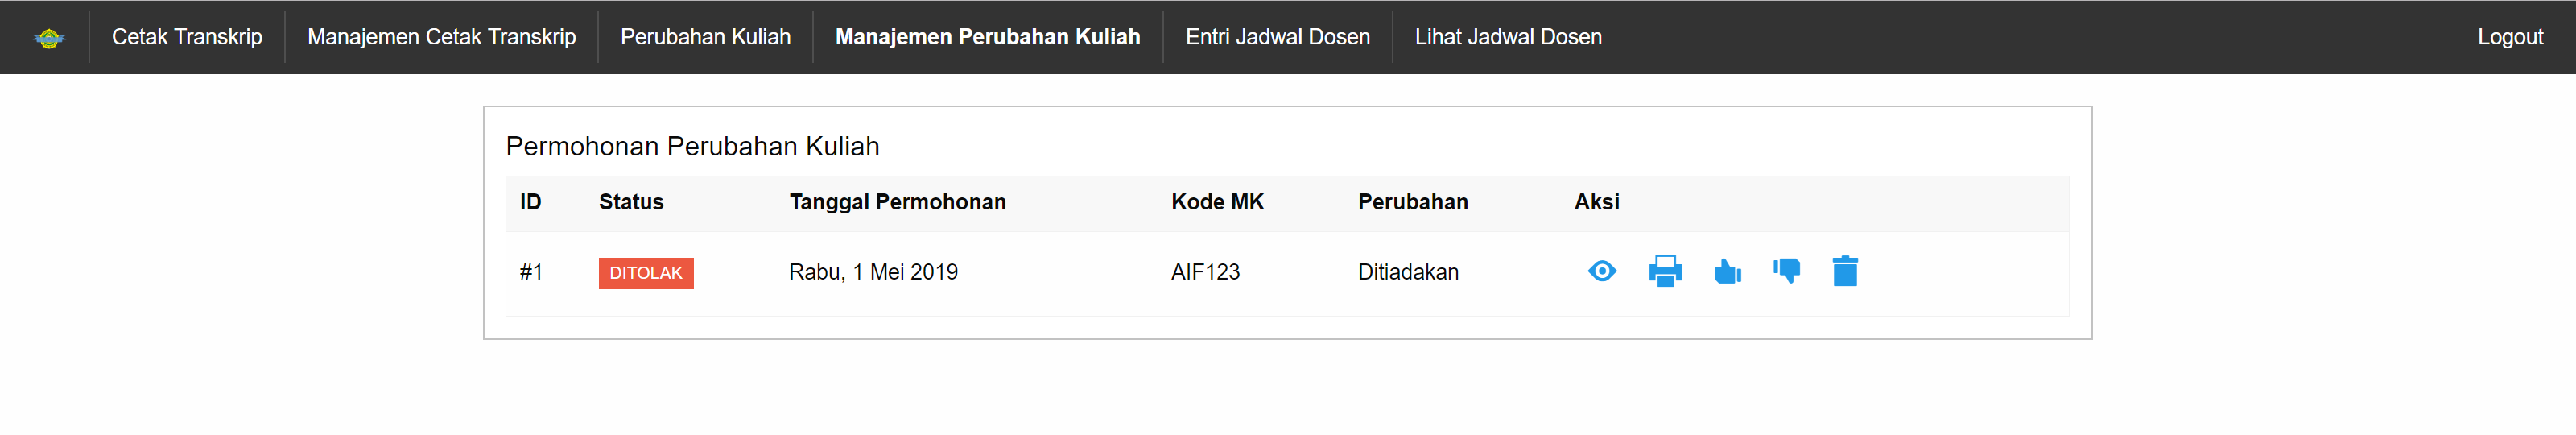
\includegraphics[scale=0.5]{Tampilan-Manajemen-Perubahan-Kuliah.png}  
	\caption{Tampilan Manajemen Perubahan Kuliah} 
\end{figure}
Tabel Pemohonan Kuliah memiliki detail yang sama dengan tabel histori permohonan, namun aksi yang dilakukan terdiri dari lima perintah:

\begin{tabular}{|p{4cm}|p{2cm}|p{10cm}|}
	\hline
	Nama Kolom & Pilihan & Keterangan\\
	\hline
	\texttt{Status} & dikonfirmasi, menggunakan kelas \colorbox{mygray}{\verb|success|} & Apabila staf TU menyetujui permohonanan\\
	\hline
	&  ditolak, menggunakan kelas \colorbox{mygray}{\verb|alert|}  & Apabila staf TU menolak permohonanan\\
	\hline
	& ditunggu, menggunakan kelas \colorbox{mygray}{\verb|secondary|} &  Apabila staf TU belum konfirmasi permohonan \\
	\hline
	\texttt{Tanggal Permohonan}    & & Data bertipe tanggal dengan format yang sudah ditentukan\\
	\hline
	\texttt{Kode MK} &  & Menampilkan data berbentuk text \\
	\hline
	\texttt{Perubahan} &  & Menampilkan data berbentuk text \\
	\hline
	\texttt{Tanggal Jawab} &  & Menampilkan data bertipe tanggal \\
	\hline
	\texttt{Keterangan} &  & Menampilkan data berbentuk text \\
	\hline
	\texttt{Aksi} & ikon \texttt{Lihat} & Ikon menggunakan font awesome dan kelas  \colorbox{mygray}{\verb|fas fa-eye|} yang akan memanggil sebuah modal sesuai id yang diinginkan user. Untuk modal, menggunakan kelas \texttt{reveal} dan atribut \texttt{data-reveal}\\
	\hline
	& ikon \texttt{Print} & Ikon menggunakan font awesome dan kelas  \colorbox{mygray}{\verb|fas fa-print|} yang akan memanggil sebuah modal sesuai id yang diinginkan user. Untuk modal, menggunakan kelas \texttt{reveal} dan atribut \texttt{data-reveal}\\
	\hline
	& ikon \texttt{Setuju} & Ikon menggunakan font awesome dan kelas  \colorbox{mygray}{\verb|fa-thumbs-up|} yang akan memanggil sebuah modal sesuai id yang diinginkan user. Untuk modal, menggunakan kelas \texttt{reveal} dan atribut \texttt{data-reveal}\\
	\hline
	& ikon \texttt{Tolak} & Ikon menggunakan font awesome dan kelas  \colorbox{mygray}{\verb|fa-thumbs-down|} yang akan memanggil sebuah modal sesuai id yang diinginkan user. Untuk modal, menggunakan kelas \texttt{reveal} dan atribut \texttt{data-reveal}\\
	\hline
	& ikon \texttt{Hapus} & Ikon menggunakan font awesome dan kelas  \colorbox{mygray}{\verb|fas fa-trash|} yang akan memanggil sebuah modal sesuai id yang diinginkan user. Untuk modal, menggunakan kelas \texttt{reveal} dan atribut \texttt{data-reveal}\\	
	\hline
\end{tabular}
\begin{figure} [H]
	\centering  
	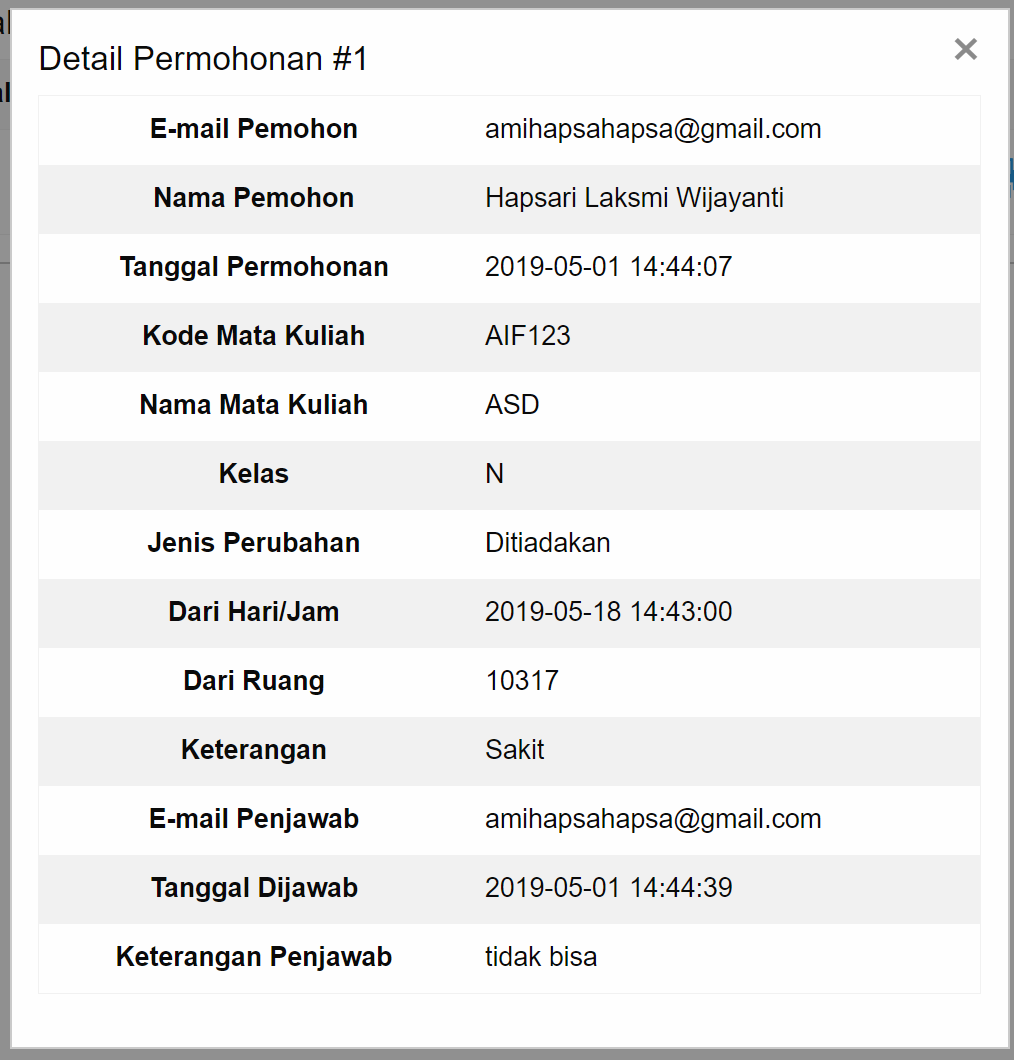
\includegraphics[scale=0.3]{Modal-Lihat-Manajemen-Perubahan-Kuliah.png}  
	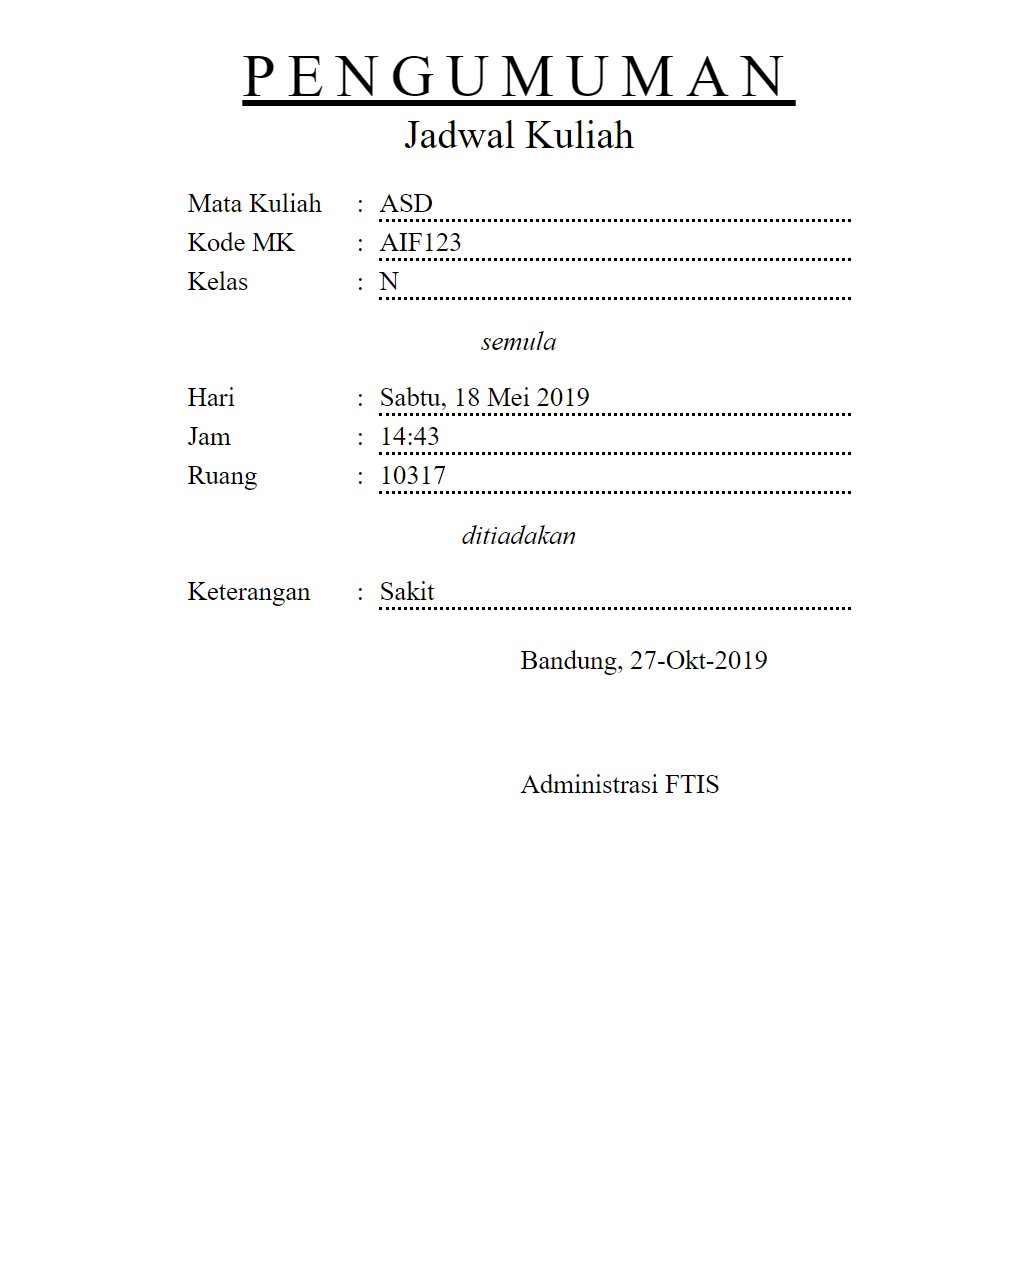
\includegraphics[scale=0.3]{Modal-Print-Manajemen-Perubahan-Kuliah.png} 
	\caption{Modal aksi Lihat dan Print Manajemen Perubahan Kuliah} 
\end{figure}


\begin{figure} [H]
	\centering  
	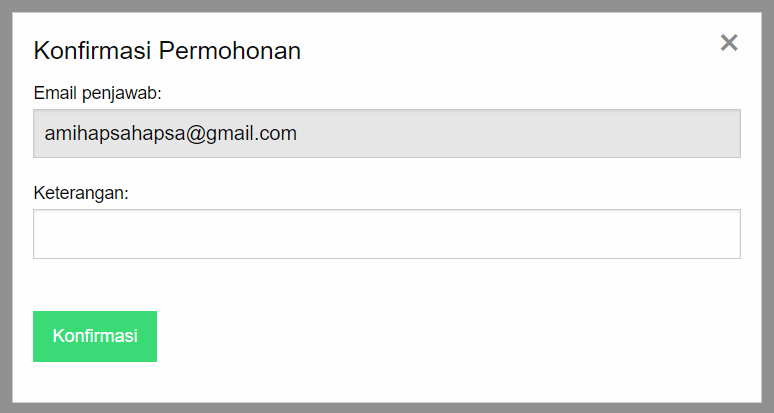
\includegraphics[scale=0.3]{Modal-Setuju-Manajemen-Perubahan-Kuliah.png}
	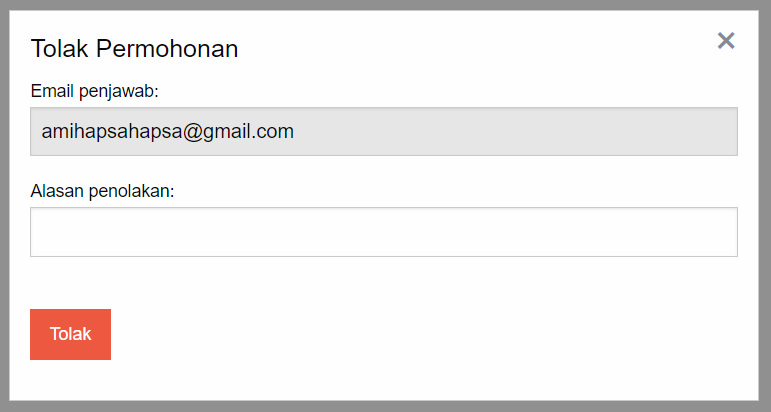
\includegraphics[scale=0.3]{Modal-Tolak-Manajemen-Perubahan-Kuliah.png}    
	\caption{Modal aksi Setuju dan Tolak Manajemen Perubahan Kuliah} 
\end{figure}


\begin{figure} [H]
	\centering  
	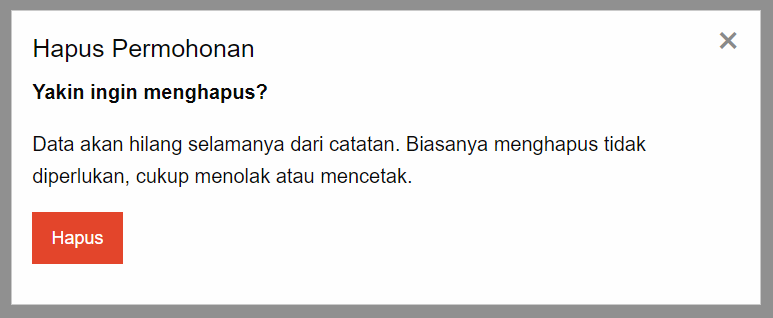
\includegraphics[scale=0.3]{Modal-Hapus-Manajemen-Perubahan-Kuliah.png}  
	\caption{Modal Hapus Manajemen Perubahan Kuliah} 
\end{figure}

Berikut ini penjelasan masing - masing modal.
\begin{enumerate}
	
	\item Modal Lihat : Terdiri dari sebuah tabel yang menampilkan data tabel permohonan. Ikon menggunakan kelas  \colorbox{mygray}{\texttt{fi-eye}} dan menerapkan atribut  \colorbox{mygray}{\texttt{data-open}} yang berisi method hapus menuju ID tertentu.
	
	\item Modal Print : Terdiri dari sebuah form yang terdiri dari label, field dan tombol berwarna biru sehingga membutuhkan kelas  \colorbox{mygray}{\verb|input-group-field|}.Ikon menggunakan kelas  \colorbox{mygray}{\texttt{fi-print}} dan menerapkan atribut \texttt{data-open} yang berisi method cetak menuju ID tertentu.
	
	\item Modal Setuju : Terdiri dari sebuah \texttt{table} yang menampilkan data permintaan transkrip. Ikon menggunakan kelas  \colorbox{mygray}{\texttt{fi-eye}} dan menerapkan atribut  \colorbox{mygray}{\texttt{data-open}} yang berisi method hapus menuju ID tertentu.
	
	\item Modal Tolak : Terdiri dari sebuah \textit{form} yang memiliki method \texttt{POST} yang memanggil sebuah method "/TranskripManage/answer". Terdapat tiga tipe input yang digunakan yaitu  \colorbox{mygray}{\texttt{hidden, text, submit}}. Pada input text untuk label Alasan Penolakan, menggunakan kelas "input-group-field". Lalu untuk input bertipe  \colorbox{mygray}{\texttt{submit}} menggunakan kelas alert-button untuk membuat button berwarna merah. Ikon menggunakan kelas \texttt{fi-dislike} dan menerapkan atribut  \colorbox{mygray}{\texttt{data-open}} yang berisi method tolak menuju ID tertentu.	
	
	\item Modal Hapus : Terdiri dari sebuah form yang terdiri dari paragraf yang bersifat bold, beberapa input dan tombol berwarna merah sehingga membutuhkan kelas \colorbox{mygray}{\texttt{<p>}}, \colorbox{mygray}{\texttt{<strong>}} dan \colorbox{mygray}{\texttt{<input>}}. Ikon menggunakan kelas  \colorbox{mygray}{\texttt{fi-trash}} dan menerapkan atribut \colorbox{mygray}{\texttt{data-open}} yang berisi method hapus menuju ID tertentu.
\end{enumerate}

\subsection{Antarmuka Entri Jadwal Dosen}
Antarmuka diaplikasikan pada file \textbf{BlueTape/www/application/views/EntriJadwalDosen/main.php}.
\begin{figure} [H]
	\centering  
	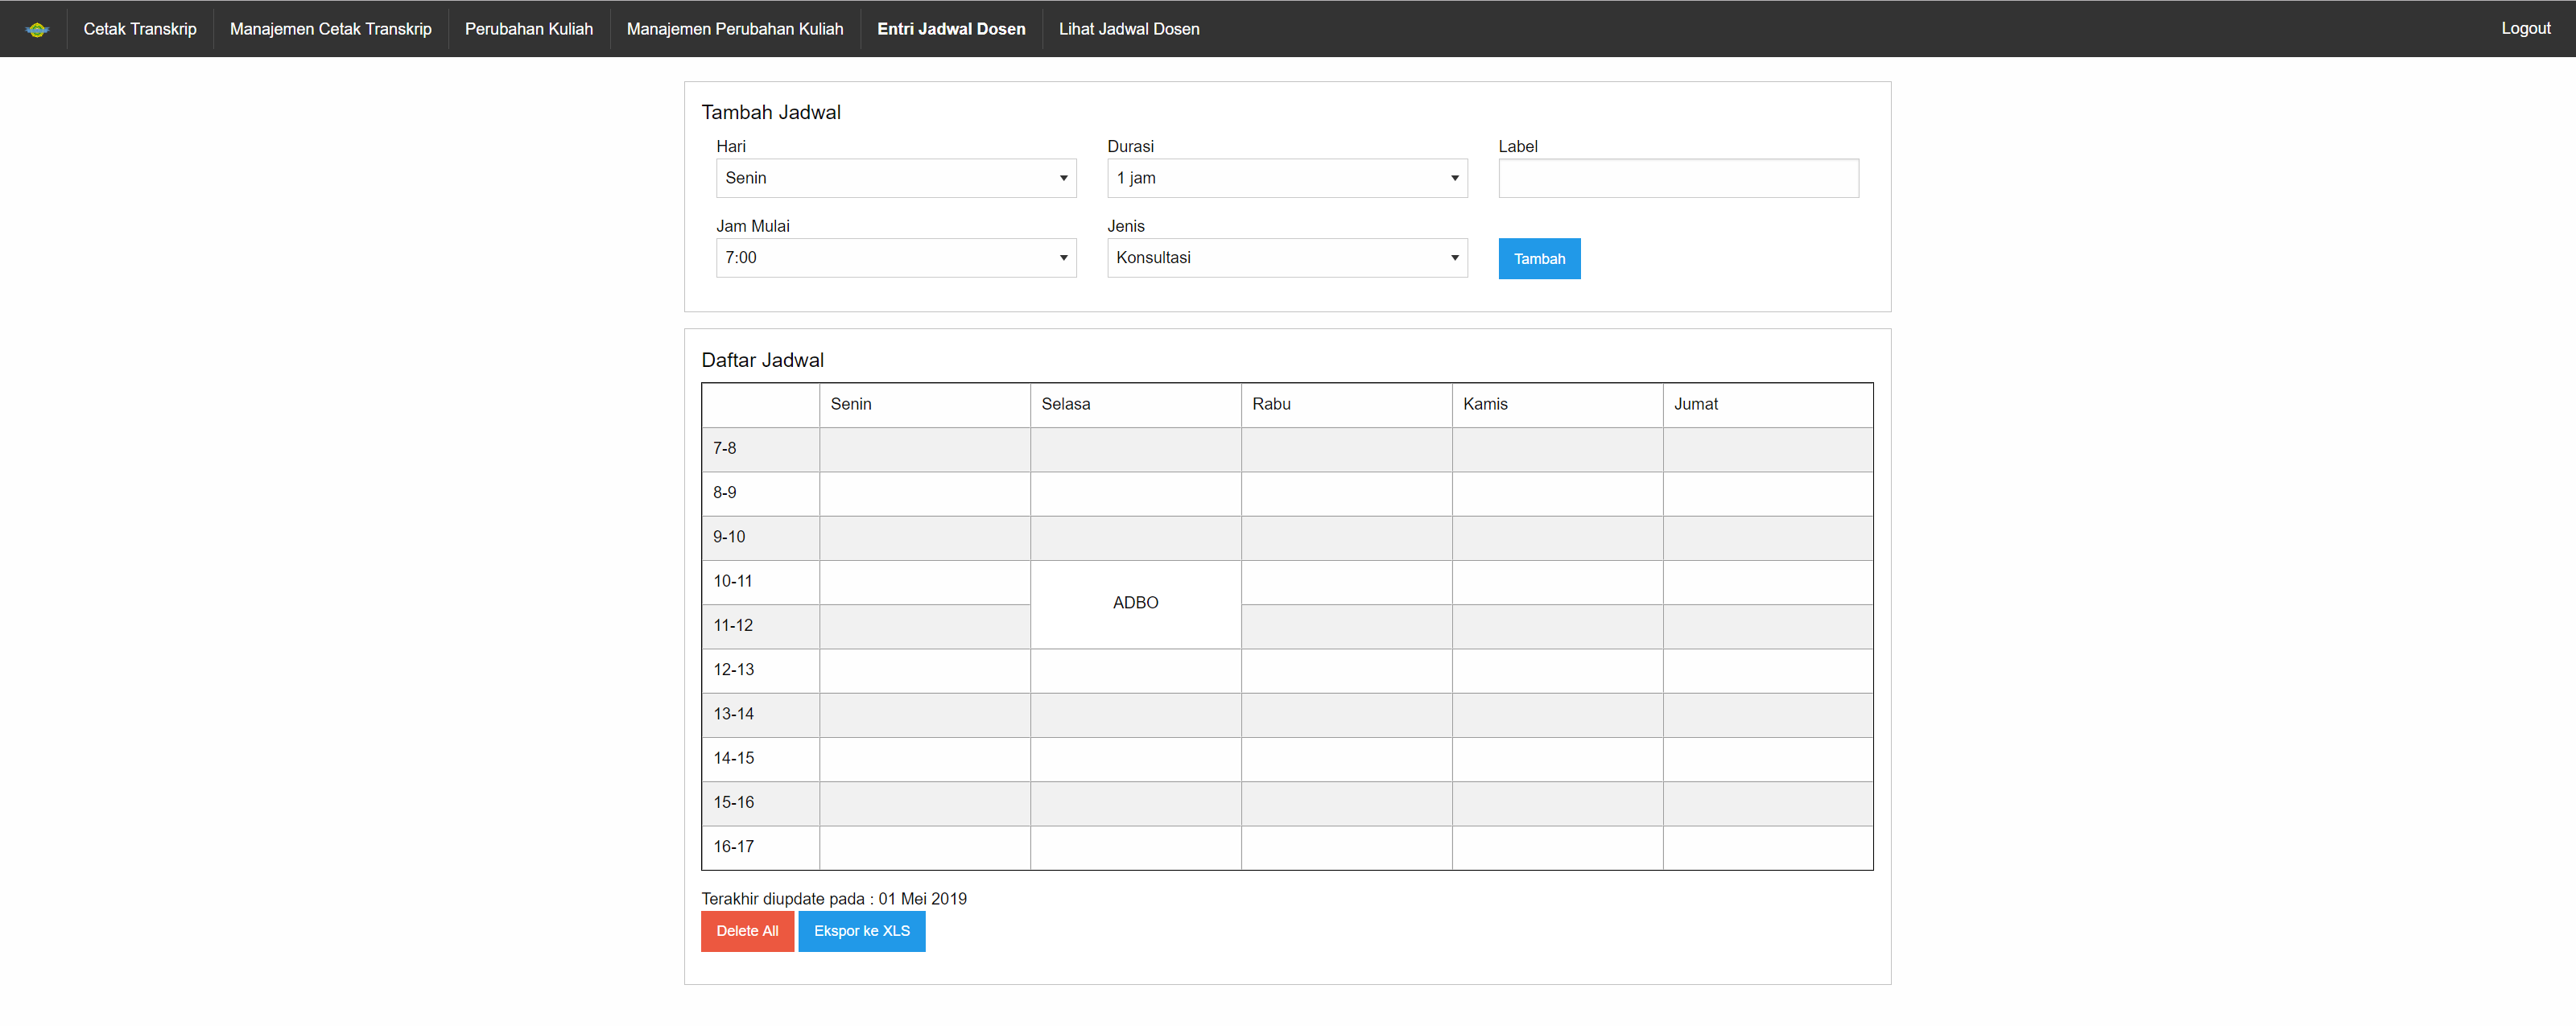
\includegraphics[scale=0.5]{Tampilan-Entri-Jadwal-Dosen.png}  
	\caption{Modal Print Manajemen Perubahan Kuliah} 
\end{figure}

Detail mengenai tabel Tambah Jadwal :
\begin{itemize}
	\item \texttt{Hari} : Terdiri dari nama hari dari senin sampai jumat.
	\item \texttt{Durasi} : Terdiri dari rentang jam kelas berlangsung dari 1 jam hingga 9 jam.
	\item \texttt{Label} : Field bertipe text.
	\item \texttt{Jam Mulai} : Terdiri dari jam dari rentang 07:00 sampai 16:00.
	\item \texttt{Jenis} : Terdiri dari tiga macam pilihan 
	\begin{enumerate}
		\item Konsultasi : Memiliki background berwarna hijau.
		\item Terjadwal : Memiliki background berwarna biru.
		\item Kelas : Memiliki background putih.
	\end{enumerate}
\end{itemize}

Desain antarmuka sebagai berikut : \par
Konten "Tambah Jadwal" dan "Daftar Jadwal" akan diletakkan pada satu \textit{row} yang memiliki kolom sebesar 12 grid pada layar medium dengan menggunakan komponen \colorbox{mygray}{\texttt{large-12 column}}, untuk setiap konten nya akan dipisahkan oleh panel yang disebut dengan \colorbox{mygray}{\texttt{callout}}. \par
Untuk konten \texttt{Tambah Jadwal} :
\begin{itemize}
	\item \texttt{Hari} : Penggunaan tag \colorbox{mygray}{\texttt{<select>}} dan \colorbox{mygray}{\texttt{<option>}}.
	\item \texttt{Jam Mulai} : Penggunaan tag \colorbox{mygray}{\texttt{<select>}} dan \texttt{<option>}.
	\item \texttt{Durasi} : Penggunaan tag \colorbox{mygray}{\texttt{large-4 columns}}
\end{itemize}


Tabel Daftar jadwal akan \textit{retrieve} data jadwal dari dosen yang dibuat. Terdiri dari rentang waktu dan hari. Jadwal yang terlihat pada tabel ini bisa diedit dan dihapus. Menggunakan kelas \colorbox{mygray}{\texttt{large-12 column}}, \colorbox{mygray}{\texttt{.callout}} dan \texttt{table-scroll}.
Dibagian bawah tabel akan terlihat tanggal jadwal tersebut di update dan memiliki dua tombol :
\begin{itemize}
	\item \texttt{Delete All} : Menghapus semua jadwal yang sudah dibuat, tombol berwarna merah dengan menerapkan kelas \colorbox{mygray}{\texttt{.alert}}.
	\item \texttt{Export ke XLS} : Secara otomatis akan membuat file excel dan mendownload di device secara lokal.Ttombol berwarna biru dengan menerapkan kelas \texttt{button}.
\end{itemize}
Setiap data yang ditampilkan bisa diedit atau hapus, apabila ditekan maka sebuah modal akan muncul.  
\begin{figure} [H]
	\centering  
	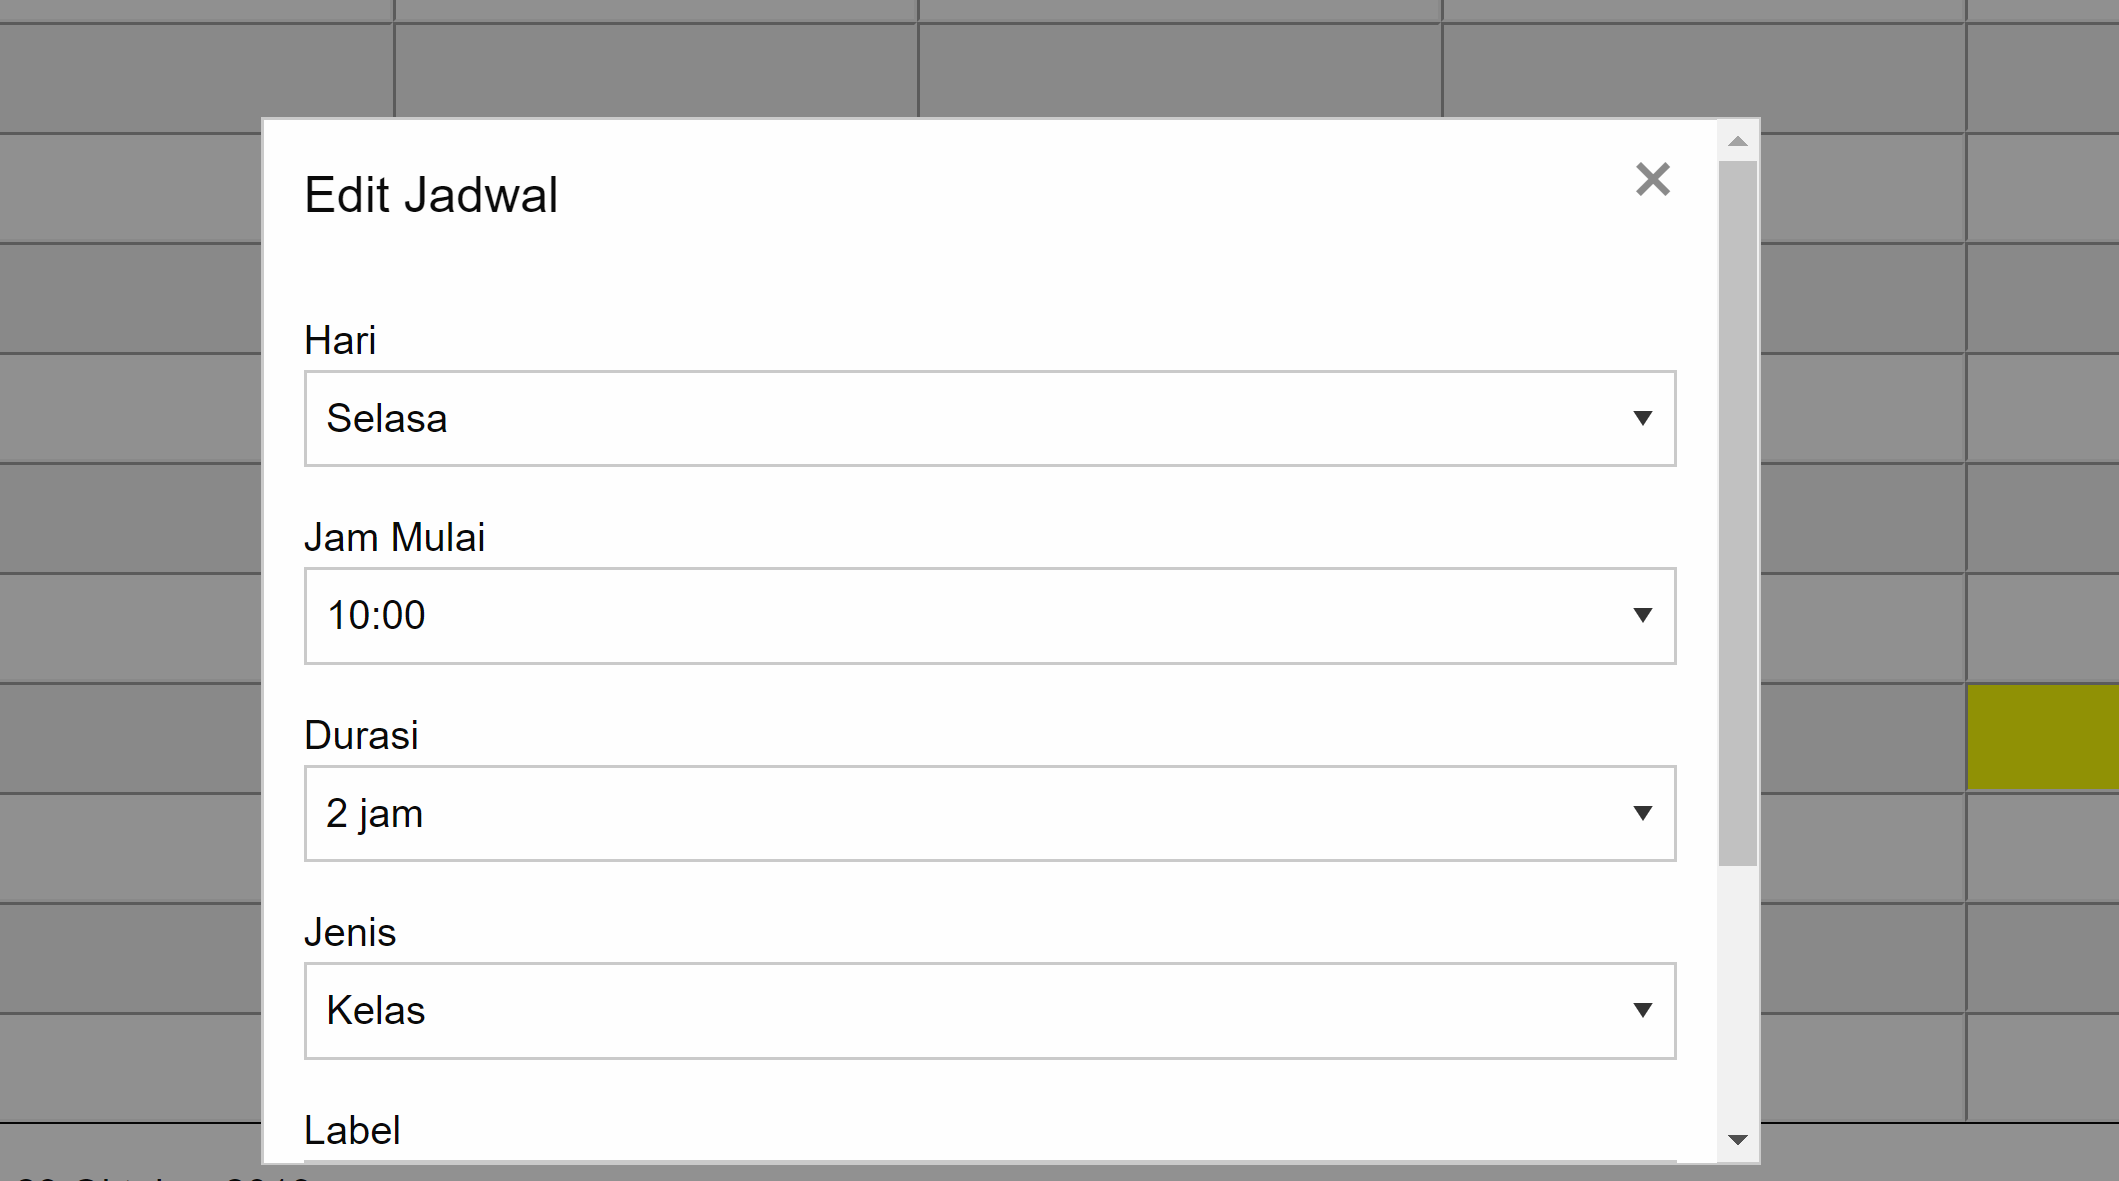
\includegraphics[scale=0.5]{Modal-Daftar-Jadwal-zurb.png}  
	\caption{} 	
\end{figure}
Modal merupakan sebuah form dengan metode "POST". Untuk field \texttt{Hari, Jam Mulai, Durasi, Jenis} dan \texttt{label} memiliki input bertipe \colorbox{mygray}{\texttt{select}}. Lalu terdapat dua button \texttt{Save} dan \texttt{Submit} yang masing - masing menggunakan kelas tag \colorbox{mygray}{\texttt{<button>}} dan \colorbox{mygray}{\texttt{.alert}}.

\subsection{Antarmuka Lihat Jadwal Dosen}
Antarmuka diaplikasikan pada file \textbf{BlueTape/www/application/views/LihatJadwalDosen/main.php}.
\begin{figure} [H]
	\centering  
	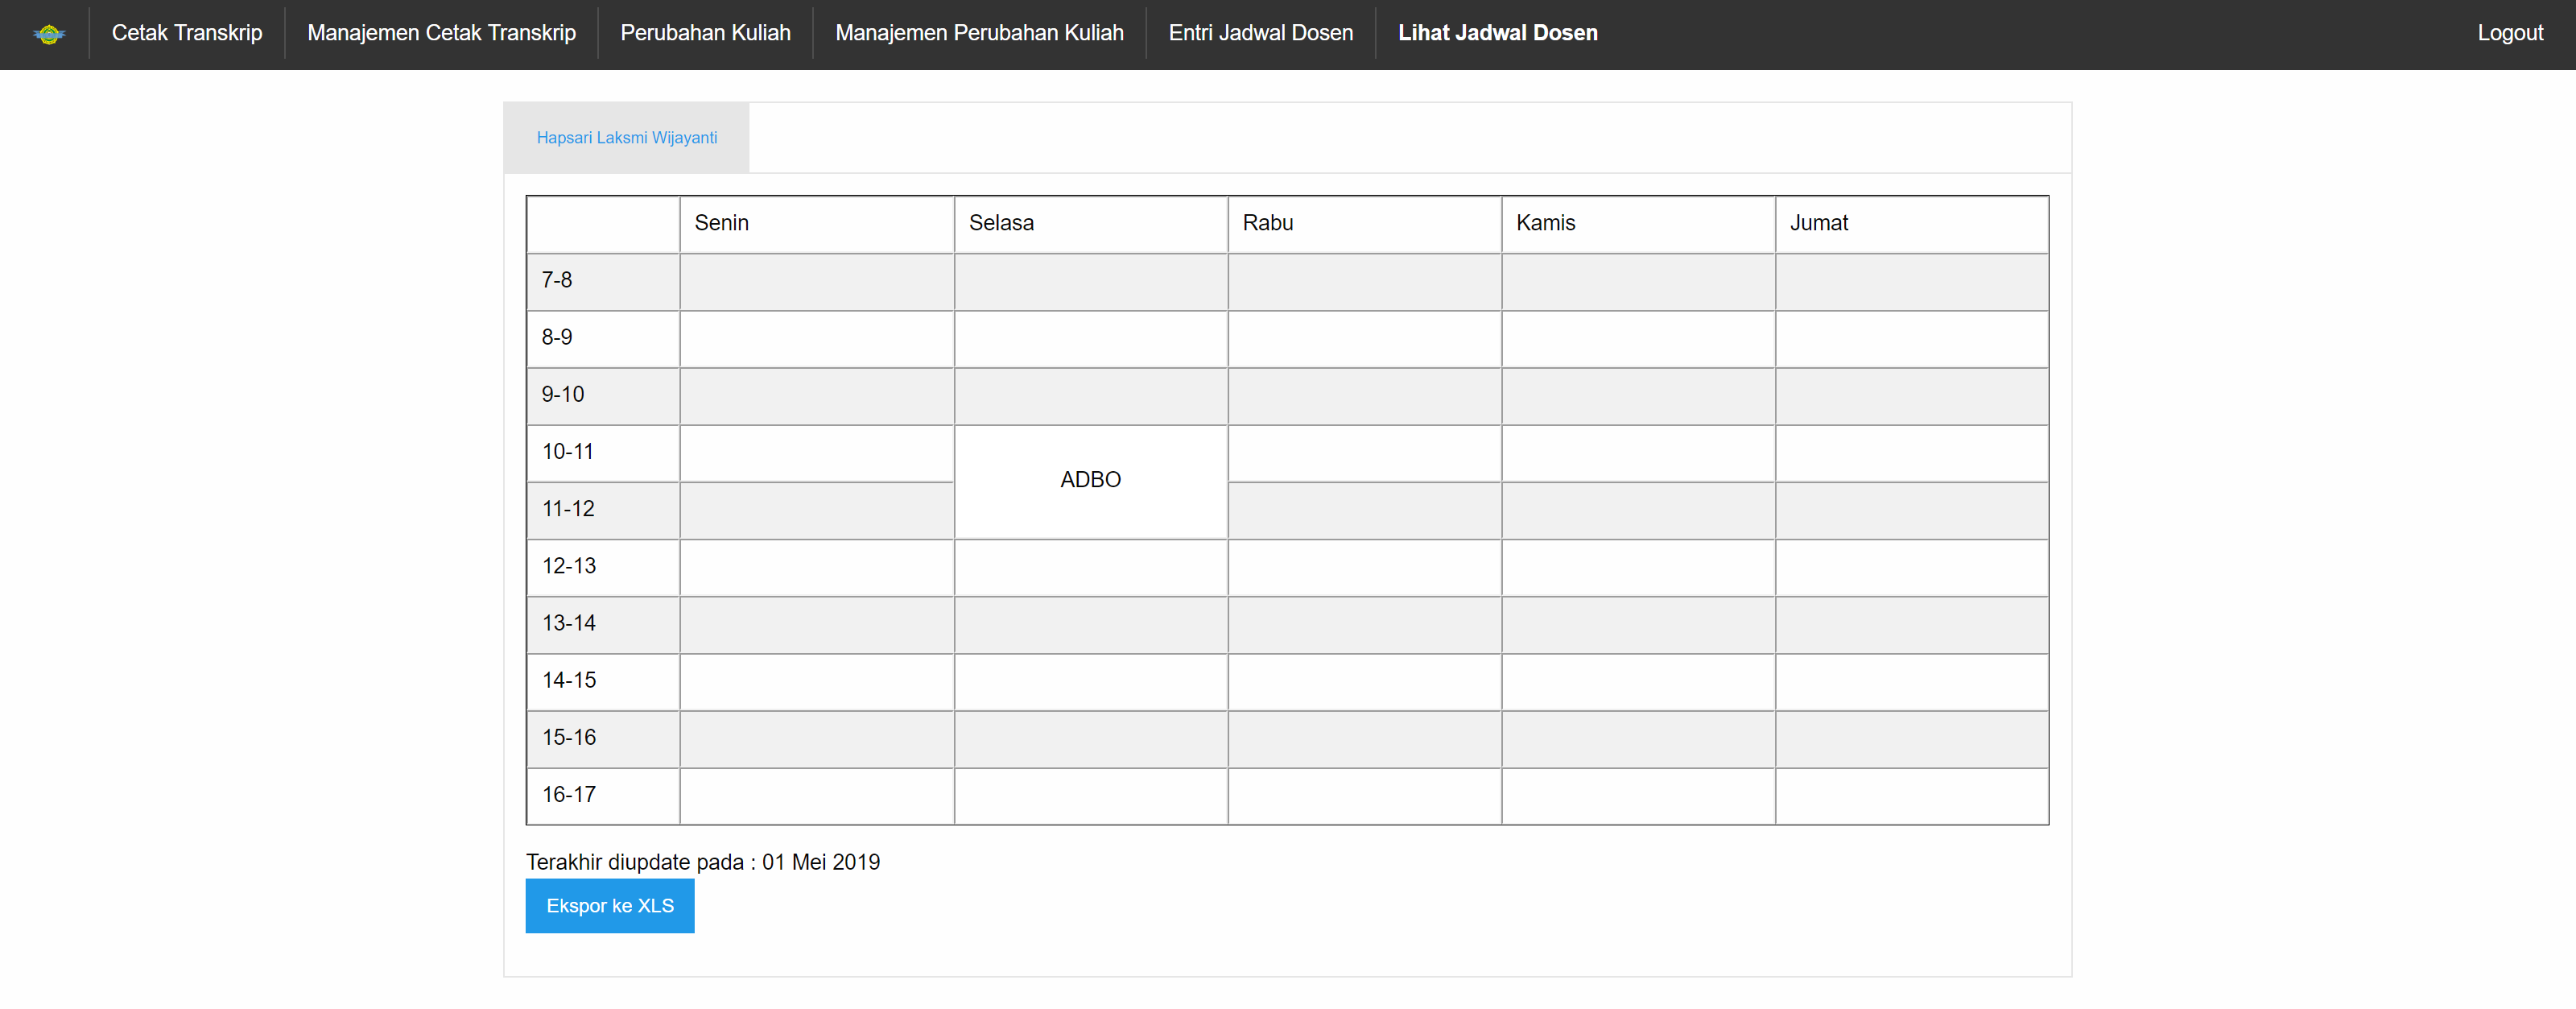
\includegraphics[scale=0.5]{Tampilan-Lihat-Jadwal-Dosen.png}  
	\caption{Struktur File Zurb Foundation} 	
\end{figure}
Tabel Jadwal Dosen terdiri dari list nama dosen yang dibuat dalam bentuk tabs sehingga menggunakan kelas \colorbox{mygray}{\texttt{tabs-panel}}. Apabila dipilih sebuah tabs maka tabel akan menampilkan data jadwal dosen.  Terdiri dari rentang waktu dan hari. Dibagian bawah tabel terdapat tanggal kapan terakhir jadwal dibuat dan tombol "Ekspor ke XLS".
